%
% chapter.tex -- Anwendungen von wahrscheinlichkeitsmatrizen
%
% (c) 2020 Prof Dr Andreas Müller, Hochschule Rapperswil
%
\chapter{Wahrscheinlichkeitsmatrizen
\label{buch:chapter:wahrscheinlichkeit}}
\lhead{Wahrscheinlichkeitsmatrizen}
\rhead{}
Matrizen beschreiben lineare Abbildungen, also einen Prozess, der
jedem Vektor einen neuen Vektor zuordnet.
Es ist daher nicht abwegig zu erwarten, dass sich 
die Zeitentwicklung eines vom Zufall beeinflussten Systems, welches sich
in mehreren verschiedenen Zuständen befinden kann, ebenfalls mit Hilfe
von Matrizen beschreiben lässt.
Eine solche Beschreiben ermöglicht leicht Verteilungen,
Erwartungswerte und stationäre Zustände zu ermitteln.

Im Abschnitt~\ref{buch:section:google-matrix} wird an Hand der Google
Matrix bezeigt, wie ein anschauliches Beispiel in natürlicher Weise
auf eine Matrix führt.
Abschnitt~\ref{buch:section:diskrete-markov-ketten} stellt dann die abstrakte
mathematische Theorie der Markov-Ketten dar und behandelt einige wichtige
Eigenschaften von Wahrscheinlichkeitsmatrizen.
Es stellt sich heraus, dass thermodynamische Quantensysteme sehr gut
mit solchen Matrizen beschrieben werden können, zum Beispiel kann man
einfache Formen von Laser auf diese Art behandeln.
Aus einem solchen System hat Parrondo ein System abgeleitet, welches 
ziemlich unerwartetes Verhalten an den Tag gelegt hat, welches mit
Hilfe von Matrizen leicht zu analysieren ist. 
Dies wird in Abschnitt~\ref{buch:section:paradoxon-von-parrondo}
dargestellt.

%
% google.tex -- Einstiegsproblem zur Behandlung von Google-Matrizen
%
% (c) 2020 Prof Dr Andreas Müller, Hochschule Rapperswil
%
\section{Google-Matrix
\label{buch:section:google-matrix}}
\rhead{Google-Matrix}
Das Internet besteht aus einer grossen Zahl von Websites, etwa 400~Millionen
aktiven Websites, jede besteht aus vielen einzelnen Seiten.
Es ist daher angemessen von $N\approx 10^9$ verschiedenen Seiten auszugehen.
Eine natürliche Sprache umfasst dagegen nur einige 100000 bis Millionen
von Wörtern.
Ein durchschnittlicher Sprecher englischer Muttersprache verwendet nur etwa
50000 Wörter.
Die Zahl der Wörter, die auf den $N$ Seiten vorkommen können, ist also
viel kleiner als die Zahl der zur Verfügung stehenden Wörter.
Ein einzelnes Wort wird daher notwendigerweise auf einer grossen Zahl
von Seiten vorkommen.
Eine Suche nach einem bestimmten Wort wird also in der überwiegenden Zahl
der Fälle derart viele Treffer zurückgeben, dass das Suchresultat
nur dann nützlich sein kann, wenn eine zusätzliche Informationsquelle
ermöglicht, die Treffer in eine sinnvolle Ordnung zu bringem.

Genau dieses Problem stellte sich den vielen traditionellen Suchmaschienen
in der ersten grossen Boomphase des Internets.
Traditionelle Informatione-Retrieval-Systeme operieren auf einem relativ
kleinen Dokumentbestand und gehen davon aus, dass bereits wenige, spezifische
Wörter nur in einem kleinen Teil des Dokumentbestandes vorkommen und damit
eine übersichtliche Treffermenge ergeben.
Die Einengung der Treffermenge dank der Suche nach spezifischer Menge
bedeutet aber auch, dass nach Synonymen oder alternative Formen eines
Wortes separat gesucht werden muss, was die Übersichtlichkeit wieder
zerstört.

%
% Ein Modell für Webseitenbesucher
%
\subsection{Ein Modell für Webseitenbesucher
\label{buch:subsection:modell-fuer-webseitenbesucher}}
\begin{figure}
\centering
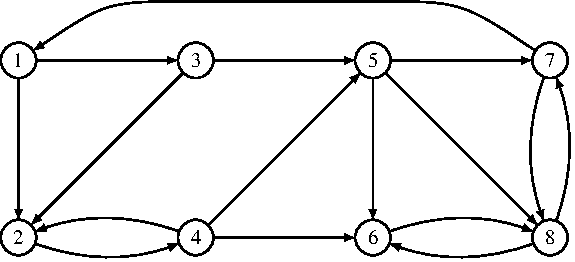
\includegraphics{chapters/80-wahrscheinlichkeit/images/internet.pdf}
\caption{Modell-Internet als Beispiel für die Link-Matrix und die Google-Matrix.
\label{buch:figure:modellinternet}}
\end{figure}

Das kombinierte Vorkommen von Wörtern oder Begriffen alleine kann also 
nicht ausreichen, um die Seiten zum Beispiel einem Fachgebiet zuzuordnen.
Dazu muss eine externe Informationsquelle angezapft werden.
Bei traditionellen Dokumenten liefert der Kontext, in dem ein
Dokument erfasst wurde, solche ergänzenden Informationen.
Eine Publikation in einem Fachjournal ordnet einen Text einem Fachgebiet zu.
Im World-Wide-Web liefert die Link-Struktur diesen Kontext.
Dokumente zu ähnlichen Themen werden bevorzugt untereinander verlinkt
sein.

Gesucht ist jetzt also ein Modell, welches objektiv die Linkstruktur
bewertet und daraus eine Rangordnung der passenden Wörter ableitet.
Die Linkstruktur kann natürlich als gerichteter Graph betrachtet und 
mit Hilfe der Matrix~\eqref{buch:graphen:eqn:linkmatrix}
beschrieben werden.
Dies trägt jedoch der Anzahl der Wahlmöglichkeiten nicht Rechnung.
Eine Website mit nur einem Link auf die Seite $j$ hat mehr Gewicht
als eine Seite mit vielen Links, unter denen der Link auf die Seite $j$
einer von vielen ist.
Im Beispiel-Inter der Abbildung~\ref{buch:figure:modellinternet}
signalisiert die Seite $t$ mit nur einem Link auf die Seite $8$
viel deutlicher, dass $8$ eine wichtige Seite ist, also die die
Seite $5$ tut, die auch noch zwei andere Links enthält.
Wir können diesen Unterschied berücksichtigen, indem wir zu einem
Wahrscheinlichkeitsmodell übergehen, was wir im folgenden Abschnitt
tun werden.


%
% Wahrscheinlichkeitsinterpretation
%
\subsection{Wahrscheinlichkeitsinterpretation
\label{buch:subsection:wahrscheinlichkeitsinterpretation}}
Ein Internetbesucher kann eine grosse Zahl von Seiten besuchen.
In diesem Abschnitt soll ein Modell entwickelt werden, welches die
Wahrscheinlichkeit zu ermitteln gestattet, dass der Besucher auf
einer bestimmten Seite landet.

\subsubsection{Ereignisse und Wahrscheinlichkeiten}
Wir bezeichnen mit $S_i$ das Ereignis, dass sich der Besucher auf
der Seite mit der Nummer $i$ befindet, wobei $i=1,\dots,N$.
Gesucht ist die Wahrscheinlichkeit $P(S_i)$.
Ohne weitere Information müssten wir davon ausgehen, dass jede Seite
etwa gleich wahrscheinlich ist, dass also $P(S_i) = 1/N$.

Wir wissen jedoch mehr.
Wir wissen, dass der Besucher die verschiedenen Seiten zu einem guten 
Teil dadurch findet, dass er Links folgt.
Die Wahrscheinlichkeit $P(S_i)$ verändert sich also, wenn die Zahl der
Links ansteigt, die auf die Seite $i$ verweisen.
Zur Beschreibung dieses Phänomens brauchen wir die zusätzliche Ereignisse
$S_i'$, die mit Wahrscheinlichkeit $P(S'_i)$ eintreten, wenn sich der
Besucher nach Navigation entlang eines Links auf der Seite $i$ befindet.

Wir nehmen jetzt zusätzlich an, dass eine grosse Zahl von Besuchern über
lange Zeit ungefähr nach den gleichen Dingen suchen und sich daher
auf die gleiche Weise auf den verschiedenen Seiten verteilen und dass
insbesondere die Verteilung stationär ist, dass also $P(S_i) = P(S'_i)$
gilt.
Suchmaschinen wie Google gehen davon aus, dass alle Besucher ungefähr
die gleichen Suchprioritäten haben, so dass es sich lohnt, die Suchresultate
nach der Wahrscheinlichkeit $P(S_i)$ zu ordnen und dem Suchenden die
wahrscheinlichsten Dokumente als erste zu zeigen.

\subsubsection{Bedingte Wahrscheinlichkeit}
Um einen Zusammenhang zwischen $P(S_i)$ und $P(S'_j)$ herzustellen, muss
die Navigation entlang der Links modelliert werden.
Die naheliegende Wahrscheinlichkeitsinterpretation ist die bedingte
Wahrscheinlichkeit $P(S'_j|S_i)$ dass der Besucher auf der Seite $j$
landet, nachdem er auf der Seite $i$ die Linknavigation verwendet hat.
Wenn es keinen Link zwischen den Seiten $i$ und $j$ gibt, dann ist diese
Navigation natürlich nicht möglich und es folgt $P(S'_j|S_i)=0$.
Falls es einen Link gibt, ist $P(S'_j|S_i)\ge 0$.

A priori wissen wir nicht, wie wahrscheinlich es ist, dass der Besucher
dem Link auf die Seite $j$ folgt, normalerweise werden nicht alle
Links mit gleicher Wahrscheinlichkeit verwendet.
Wir nehmen daher zusätzlich an, dass alle Links gleich wahrscheinlich
sind.
Die Seite $i$ enthält $n_i$ Links, also ist die Wahrscheinlichkeit,
auf einer von $i$ aus verlinkten Seite $j$ zu landen $P(S'_j|S_i) = 1/n_i$.

\subsubsection{Totale Wahrscheinlichkeit}
Der Satz von der totalen Wahrscheinlichkeit ermöglicht, einen Zusammenhang
\index{totale Wahrscheinlichkeit}%
\index{Wahrscheinlichkeit!totale}%
zwischen $P(S'_j)$ und $P(S_i)$ herzustellen.
Es gilt
\begin{equation}
P(S'_j)
=
P(S'j|S_1) P(S_1)
+
P(S'j|S_2) P(S_2)
+
\dots
+
P(S'j|S_N) P(S_N).
\label{buch:google:eqn:totalewahrscheinlichkeit}
\end{equation}
Dies kann in Matrix- und Vektorform übersichtlicher geschrieben werden.
Dazu fassen wir die Wahrscheinlichkeiten $p'_j=P(S'_j)$ und $p_i=P(S_i)$
also Vektoren
\[
p
=
\begin{pmatrix}
P(S_1)\\
P(S_2)\\
\vdots\\
P(S_N)
\end{pmatrix}
\qquad
\text{und}
\qquad
p'
=
\begin{pmatrix}
P(S'_1)\\
P(S'_2)\\
\vdots\\
P(S'_N)
\end{pmatrix}
\]
zusammen.
Die bedingten Wahrscheinlichkeiten $h_{ji}=P(S'_j|S_i)$ sind mit zwei Indizes
beschrieben, sie bilden daher in natürlicher Weise eine Matrix
\[
H
=
\begin{pmatrix}
P(S'_1|S_1)&P(S'_1|S_2)&\dots &P(S'_1|S_N)\\
P(S'_2|S_1)&P(S'_2|S_2)&\dots &P(S'_2|S_N)\\
\vdots     &\vdots     &\ddots&\vdots     \\
P(S'_N|S_1)&P(S'_N|S_2)&\dots &P(S'_N|S_N)
\end{pmatrix}.
\]
Die Formel~\eqref{buch:google:eqn:totalewahrscheinlichkeit} wird dann zur
Formel für das Produkt Matrix mal Vektor:
\[
(Hp)_j
=
\sum_{i=1}^N h_{ji} p_i
=
\sum_{i=1}^N P(S'_j|S_i) P(S_i)
=
p'_j
\qquad\Rightarrow\qquad
Hp=p'.
\]
Die Matrix $H$ modelliert also die Wahrscheinlichkeit der Navigation
entlang eines Links.

\begin{beispiel}
Für das Beispiel-Internet von Abbildung~\ref{buch:figure:modellinternet}
ist die zugehörige Matrix
\begin{equation}
H =
\begin{pmatrix}
   0   & 0&   0   &   0   &   0   & 0&\frac12&   0   \\
\frac12& 0&\frac12&\frac13&   0   & 0&   0   &   0   \\
\frac12& 0&   0   &   0   &   0   & 0&   0   &   0   \\
   0   & 1&   0   &   0   &   0   & 0&   0   &   0   \\
   0   & 0&\frac12&\frac13&   0   & 0&   0   &   0   \\
   0   & 0&   0   &\frac13&\frac13& 0&   0   &\frac12\\
   0   & 0&   0   &   0   &\frac13& 0&   0   &\frac12\\
   0   & 0&   0   &   0   &\frac13& 1&\frac12&   0
\end{pmatrix}.
\label{buch:google:eqn:linkmatrixbeispiel}
\end{equation}
\qedhere
\end{beispiel}

%
% Freier Wille
%
\subsection{``Freier Wille''
\label{buch:subsection:freier-wille}}
Das Modell in
Abschnitt~\eqref{buch:subsection:wahrscheinlichkeitsinterpretation}
beschriebene Modell geht unter anderem davon aus, dass der Benutzer
ausschliesslich die Navigation entlang der Links verwendet.
Natürlich gibt es viele weitere Wege, auf denen ein Besucher auf einer
bestimmten Seite landen kann.
Er kann zum Beispiel einen Link auf eine Seite per Email zugesandt
erhalten haben.
Ein solcher Link ist nicht enthalten in einer öffentlich zugänglichen
Seite des Internets und wird daher auch von der Matrix $H$ nicht
erfasst.
Eine weitere wichtige Quelle von Links sind dynamisch erzeugte Links
wie zum Beispiel die Suchresultate einer Suchmaschine.
Hier entsteht die Möglichkeit, dass die erfolgreiche Suchmaschine,
die ihre Suchresultate unter Zuhilfenahme der Matrix $H$ sortiert,
ihr eigenes Modell, auf dem ihr Erfolg basiert, torpediert.

\subsubsection{Erweiterung der Link-Matrix}
Wir bezeichnen das Ereignis, dass der Benutzer nicht die Link-Navigation
verwendet mit $F$ für ``freier Wille'', obwohl es so etwas natürlich nicht
gibt.
Die Wahrscheinlichkeit, auf der Seite $S'_j$ zu landen, setzt sich jetzt
aus den zwei Fällen $F$ und $\overline{F}$ zusammen, für die erneut der
Satz von der totalen Wahrscheinlichkeit den Zusammenhang
\[
P(S'_j)
=
P(S'_j|\overline{F}) P(\overline{F})
+
P(S'_j|F) P(F)
\]
Die Wahrscheinlichkeit $\alpha = P(F)$, mit der der Benutzer den
``freiene Willen'' bemüht, kann experimentell durch Studien ermittelt
werden, die das Benutzerverhalten beobachten.

Die Wahrscheinlichkeit $P(S'_j|\overline{F})$ entsteht dadurch, dass
der Benutzer der Linknavigation folgt, sie entspricht also der früher
berechnenten Wahrscheinlichkeit
\[
P(S'_j|\overline{F}) = \sum_{i=1}^N P(S'_j|S_i) P(S_i).
\]
oder in Vektorform
\[
(P(S'_j|\overline{F}))_{j=1,\dots,n}
=
Hp.
\]

Über die spontane Besuchswahrscheinlichkeit $P(S'_j|F)$ wissen wir 
nichts.
Eine erste Annahme könnte sein, dass jede Seite gleich wahrscheinlich
ist, dass also $P(S'_j|F)=1/N$.
Alternativ könnte man auch eine Wahrscheinlichkeitsverteilung
$q_j = P(S'_j|F)$ experimentell zu ermitteln versuchen.
Unter der Annahme, dass alle Seitenbesuche im Falle $F$ auf Grund
eines Sucheresultats einer Suchmaschine erfolgen, könnte die
Suchmaschine den Vektor $q$ aus ihrer eigenen Suchstatistik ermitteln.

Das erweiterte Modell kann also durch
\begin{equation}
P(S'_j)
=
\sum_{i=1}^N
\alpha P(S'_j|S_i) P(S_i)
+
(1-\alpha) q_j
\qquad\Rightarrow\qquad
p'
=
\alpha Hp
+
(1-\alpha)q
\label{buch:google:eqn:composed}
\end{equation}
beschrieben werden.

\subsubsection{Die Google-Matrix}
Die Formel~\eqref{buch:google:eqn:composed} erlaubt, die Wahrscheinlichkeit
$p'$ aus $p$ und $q$ zu berechnen.
Für die Ermittlung der der stationären Verteilung war jedoch die Form
$p=Hp$ besonders nützlich, weil sie das Problem in ein Eigenwertproblem
mit einem bekanntem Eigenwert verwandelt.
Wir streben daher an, die Formel~\eqref{buch:google:eqn:composed}
ebenfalls in die Form $p=Gp$ mit einer neuen Matrix $G$ zu bringen.

Die Matrixform von
\label{buch:google:eqn:composed}
zeigt, dass sich die gesuchte Matrix $G$ zusammensetzt aus dem Summanden
$\alpha H$ und einem weiteren Summanden $A$ mit der Eigenschaft, dass
$Ap = q$ für jeden beliebigen Wahrscheinlichkeitsvektor $p$.
Da sich die Wahrscheinlichkeiten im Vektor $p$ zu $1$ summieren, gilt
\[
\underbrace{
\begin{pmatrix}
1&1&\dots&1
\end{pmatrix}
}_{\displaystyle = U^t}
\begin{pmatrix}
P(S_1)\\
P(S_2)\\
\vdots\\
P(S_N)
\end{pmatrix}
=
P(S_1)+P(S_2)+\dots+P(S_N)=1.
\]
Man erhält also die Wirkung der gewünschte Matrix $A$, indem man $p$
erst mit dem Zeilenvektor $U^t$ und das Resultat mit $q$ multipliziert.
Es gilt daher
\[
Ap = qU^tp
\qquad\Rightarrow\qquad
A=qU^t.
\]
Ausmultipliziert ist dies die Matrix
\[
A=\begin{pmatrix}
q_1&q_1&\dots&q_1\\
q_2&q_2&\dots&q_2\\
\vdots&\vdots&\ddots&\vdots\\
q_N&q_N&\dots&q_N
\end{pmatrix}.
\]
Im Fall $q=\frac1NU$ kann dies zu
\[
A
=
\frac1N UU^t
=
\frac1N
\begin{pmatrix}
1&1&\dots&1\\
1&1&\dots&1\\
\vdots&\vdots&\ddots&\vdots\\
1&1&\dots&1
\end{pmatrix}
\]
vereinfacht werden.

\begin{definition}[Google-Matrix]
Die Matrix
\begin{equation}
G
=
\alpha H
+
\frac{1-\alpha}{N}
UU^t
\qquad\text{oder}\qquad
G
=
\alpha H
+
(1-\alpha)qU^t
\label{buch:wahrscheinlichkeit:eqn:google-matrix}
\end{equation}
heisst die
{\em Google-Matrix}.
\index{Google-Matrix}%
\end{definition}

Die Google-Matrix wurde von Sergei Brin und Larry Page 
in dem Artikel \cite{BRIN1998107} als Basis der Suchmaschine
Google beschrieben.
Sie war die Basis für den Erfolg von Google und wird dem Prinzip nach
auch heute noch zur Rangierung der Suchresultate verwendet.
Dazu muss natürlich die Gleichung $p=Gp$ gelöst werden, was
weiter unten in Abschnitt~\ref{buch:subsection:wahrscheinlichkeitsverteilung}
diskutiert wird.

Natürlich ist die heutzutage verwendete Matrix mit Sicherheit komplizierter.
In der vorgestellten Form unterstützt sie zum Beispiel auch das folgende
Geschäftsmodell, welches in der Anfangszeit von Google eine Zeitlang 
erfolgreich war.
Ein Anbieter betreibt zu diesem Zweck eine grosse Zahl von Websites,
deren Seiten im Wesentlichen aus Suchbegriffen und Links untereinander
und auf die Website des Kunden verweisen.
Dadurch entsteht für die Google-Matrix der ``Eindruck'', dass sehr viele
Websites gibt, die die Kundenwebsite als relevant für die Suchbegriffe 
ansehen.
Die Kundenwebsite wird daher in den Suchresultaten weiter oben gezeigt.
Das Problem rührt natürlich daher, dass alle Links als gleichermassen
aussagekräftig betrachtet werden.

Die aktuell verwendete Variante der Google-Matrix ist natürlich ein
Betriebsgeheimnis der Firma Google.

%
% Bestimmung der zu erwartenden stationären Verteilung
%
\subsection{Wahrscheinlichkeitsverteilung
\label{buch:subsection:wahrscheinlichkeitsverteilung}}
Die Google-Matrix $G$ selbst interessiert weniger als die
Wahrscheinlichkeitsverteilung $p$.
Ziel dieses Abschnittes, ist den Vektor $p$ zu berechnen.

\subsubsection{Stationäre Verteilung}
Die Einträge $P(S_i)$ des Vektors $p$ geben die Wahrscheinlichkeit an, mit
der sich ein Benutzer auf der Seite $i$ befindet.
Wir interpretieren diese Wahrscheinlichkeit auch als ein Mass für die
Relevanz einer Seite.

Wir nehmen an, dass sich diese Wahscheinlichkeit nur langsam ändert.
Diese Annahme trifft nicht zu für neue Nachrichten, die durchaus eine
hohe Relevanz haben, für es aber noch nicht viele Links geben kann,
die die Relevanz in der Google-Matrix erkennbar machen.
Die Annahme bedeutet, dass sich die Verteilung $p$ sehr viel langsamer 
ändert als der Navigationsprozess entlang der Links erfolgt.
In erster Näherung ist es daher zulässig, nach einem Vektor $p$ zu
suchen, der sich unter Navigation nicht ändert, also nach einer
{\em stationären} Lösung.
\index{stationäre Verteilung}%

Für eine stationäre Wahrscheinlichkeitsverteilung gilt $p'=p$.
Der Vektor $p$ erfüllt daher die Gleichung
\begin{equation}
Gp = p.
\label{buch:google:ewgleichung}
\end{equation}
$p$ ist also ein Eigenvektor der Matrix $G$ zum Eigenwert $1$.

Für ein sehr kleines Netzwerk wie im oben dargestellten Beispiel ist es
einfach, mit verbreiteten numerischen Algorithmen alle Eigenwerte und
Eigenvektoren zu finden.
Benötigt wird allerdings nur der Eigenvektor zum Eigenwert $1$.

\begin{beispiel}
Ein Eigenvektor zum Eigenwert $1$ der Matrix $G$, die aus der Matrix $H$
von \eqref{buch:google:eqn:linkmatrixbeispiel}
und dem Vektor $q=\frac18u$ und $\alpha=0.9$ gebildet wurde, ist
\[
p_0=\begin{pmatrix}
   0.20100\\
   0.25440\\
   0.12163\\
   0.26014\\
   0.16394\\
   0.45543\\
   0.37739\\
   0.66007
\end{pmatrix}
\qquad\Rightarrow\qquad
p
=
\frac{1}{\|p_0\|_1}p_0
=
\begin{pmatrix}
   0.080595\\
   0.102004\\
   0.048769\\
   0.104305\\
   0.065735\\
   0.182609\\
   0.151320\\
   0.264664
\end{pmatrix}.
\]
Der Vektor $p_0$ ist ein Einheitsvektor in der euklidischen Norm.
Er kann daher nicht eine Wahrscheinlichkeitsverteilung sein,
da sich die Elemente nicht zu $1$ summieren.
Die $L^1$-Norm $\|\;\cdot\;\|_1$ eines Vektors ist die Summe der Beträge aller
Elemente eines Vektors.
Indem man $p_0$ durch die Summe aller Einträge von $p_0$ teilt,
erhält man die Wahrscheinlichkeitsverteilung $p$.
\end{beispiel}


\subsubsection{Potenzverfahren}
Die üblichen Algorithmen wie der Francis-Algorithmus zur Bestimmung
von Eigenwerten und Eigenvektoren ist für grosse Matrizen nicht praktikabel.
Da aber $1$ der betragsgrösste Eigenwert ist, kann sehr oft ein zugehöriger
Eigenvektor mit der nachfolgend beschriebenen {\em Potenzmethode}
gefunden werden.

Sei $A$ eine $n\times n$-Matrix, der Einfachheit halber nehmen wir an,
dass die Eigenwerte $\lambda_1>\lambda_2\ge \dots\ge \lambda_n$
absteigend geordnet sind,
und dass $v_1,\dots,v_n$ zugehörige linear unabhängige Eigenvektoren sind.
Ein beliebiger Vektor $v$ lässt sich in der Eigenbasis von $A$
als
\[
v = a_1v_1+\dots+a_nv_n
\]
ausdrücken.
Wendet man darauf die Matrix $A$ $k$-mal an, erhält man
\[
A^kv
=
a_1\lambda_1^k v_1 
+
a_2\lambda_2^k v_2
+
\dots
+
a_n\lambda_2^k v_n.
\]
Da $\lambda_1$ der betragsmässig grösste Eigenwert ist, wird der Vektor
$A^kv$ ungefähr mit der $k$-ten Potenz anwachsen.
Indem man durch $\lambda_1^k$ teilt, erhält man
\[
\frac{1}{\lambda_1^k} A^k v
=
a_1v_1
+
a_2\biggl(\frac{\lambda_2}{\lambda_1}\biggr)^k v_2
+
\dots
+
a_n\biggl(\frac{\lambda_n}{\lambda_1}\biggr)^k v_n.
\]
Da alle Brüche Betrag $<1$ haben, konvergiert die rechte Seite für $k\to\infty$
gegeben den  ersten Summanden.
Durch wiederholte Anwendung von $A/\lambda_1$ auf einen (fast) belieibigen
Startvektor $v$ erhält man also eine Folge von Vektoren, die gegen eine
Eigenvektor zum Eigenwert $\lambda_1$ konvergiert.

Numerische Ungenauigkeiten können bewirken, dass die Iteration mit der
Matrix $A/\lambda_1$ trotzdem nicht konvergiert.
Man kann dies komponsieren, indem man nach jeder Iteration normiert.
Da der gesuchte Eigenvektor eine Wahrscheinlichkeitsverteilung sein muss,
muss die $L^1$-Norm $1$ sein.
Statt mit der euklidischen $L^2$-Norm zu normieren, normiert man daher
besser mit der $L^1$-Norm.
Damit ergibt sich das folgende Verfahren zur Bestimmung der Pagerank-Verteilung
$p$ für die Google-Matrix.

\begin{satz}
Für die Google-Matrix $p$ konvergiert die Folge 
\[
p^{(0)} = u,
\qquad
p^{(k+1)} = \frac{G^{(k)}}{\| G^{(k)} \|_1}
\]
gegen die stationäre Verteilung $p$ mit $Gp=p$.
\end{satz}




%
% markov.tex -- diskrete Markov-Ketten und Übergangsmatrizen
%
% (c) 2020 Prof Dr Andreas Müller, Hochschule Rapperswil
%
\section{Diskrete Markov-Ketten und Wahrscheinlichkeitsmatrizen
\label{buch:section:diskrete-markov-ketten}}
\rhead{Diskrete Markov-Ketten}
Die einführend im Abschnitt~\ref{buch:section:google-matrix}
vorgestellte Google-Matrix ist nur ein Beispiel für ein
Modell eines stochastischen Prozesses, der mit Hilfe von Matrizen
modelliert werden kann.
In diesem Abschnitt soll diese Art von Prozessen etwas formalisiert
werden.

%
% Beschreibung der Markov-Eigenschaft
% 
\subsection{Markov-Eigenschaft}
% XXX Notation, Zustände, Übergangswahrscheinlichkeit
Ein stochastischer Prozess ist eine Familie von Zustandsvariablen
$X_t$ mit Werten in einer Menge $\mathcal{S}$ von Zuständen.
Der Parameter $t$ wird üblicherweise als die Zeit interpretiert,
er kann beliebige reelle Werte oder diskrete Werte annahmen, im letzten
Fall spricht man von einem Prozess mit diskreter Zeit.

Das Ereignis $\{X_t=x\}$ wird gelesen als ``zur Zeit $t$ befindet sich
der Prozess im Zustand $x$''.
Mit $P(X_t = x)$ wir die Wahrscheinlichkeit bezeichnet, dass sich
der Prozess zur Zeit $t$ im Zustand $x$ befindet.
Die Funktion $t\mapsto X_t$ beschreiben also den zeitlichen Ablauf
der vom Prozess durchlaufenen Zustände.
Dies ermöglicht, Fragen nach dem Einfluss früherer Zustände,
also des Eintretens eines Ereignisses $\{X_{t_0}=x\}$ auf das Eintreten eines
Zustands $s\in\mathcal{S}$ zu einem späteren Zeitpunkt $t_1>t_0$
zu studieren.
Das Ereignis $\{X_t = x\}$ kann man sich als abhängig von der Vorgeschichte
vorstellen.
Die Vorgeschichte besteht dabei aus dem Eintreten gewisser Ereignisse
\[
\{X_0=x_0\},
\{X_1=x_1\},
\{X_2=x_2\},
\dots,
\{X_n=x_n\}
\]
zu früheren Zeiten $t_0<t_1<\dots<t_n<t$.
Die bedingte Wahrscheinlichkeit
\begin{equation}
P(X_t = x|
X_{t_n}=x_n\wedge X_{t_{n-1}}=x_{n-1}\wedge\dots\wedge X_{t_1}=x_1\wedge
X_{t_0}=x_0)
\label{buch:wahrscheinlichkeit:eqn:historybedingt}
\end{equation}
ist die Wahrscheinlichkeit dafür, dass der Prozess zur Zeit $t$ den
Zustand $x$ erreicht, wenn er zu den Zeitpunkten $t_0,t_1,\dots,t_n$
die Zustände $x_0,x_1,\dots,x_n$ durchlaufen hat.

\subsubsection{Gedächtnislosigkeit}
% XXX Gedächtnislösigkeit, Markov-Eigenschaft
In vielen Fällen ist nur der letzte durchlaufene Zustand wichtig.
Die Zustände in den Zeitpunkten $t_0<\dots<t_{n-1}$ haben dann keinen
Einfluss auf die Wahrscheinlichkeit.
Auf die bedingte
Wahrscheinlichkeit~\eqref{buch:wahrscheinlichkeit:eqn:historybedingt}
sollten also die Ereignisse $\{X_{t_0}=x_0\}$ bis $\{X_{t_{n-1}}=x_{n-1}\}$
keinen Einfluss haben.

\begin{definition}
Ein stochastischer Prozess erfüllt die Markov-Eigenschaft, wenn 
für jede Folge von früheren Zeitpunkten $t_0<t_1<\dots <t_n<t$ und Zuständen
$x_0,\dots,x_n,x\in \mathcal{S}$ die 
Wahrscheinlichkeit~\eqref{buch:wahrscheinlichkeit:eqn:historybedingt}
nicht von der Vorgeschichte abhängt, also
\[
P(X_t = x|
X_{t_n}=x_n\wedge X_{t_{n-1}}=x_{n-1}\wedge\dots\wedge X_{t_1}=x_1\wedge
X_{t_0}=x_0)
=
P(X_t = x|
X_{t_n}=x_n).
\]
\index{Markov-Eigenschaft}
\end{definition}

Die Wahrscheinlichkeiten $P(X_t=x|X_s=y)$ mit $t>s$ bestimmen das
zeitliche Verhalten der Wahrscheinlichkeiten vollständig.
Wir schreiben daher auch
\[
p_{xy}(t, s)
=
P(X_t = x|X_s=y)
\]
für die sogenannte {\em transiente Übergangswahrscheinlichkeit}.
Für eine endliche Menge von Zuständen, können die transienten
Übergangswahrscheinlichkeiten auch als zeitabhängige 
quadratische Matrix $P(s,t)$ geschrieben werden, deren
Einträge
\[
(P(s,t))_{xy}
=
p_{xy}(t,s)
\]
mit den Zuständen $x,y\in\mathcal{S}$ indiziert sind.

\subsubsection{Die Chapman-Kolmogorov-Gleichung}
% XXX Chapman-Kolmogorov-Gleichung
Man beachte, dass in der Definition der Markov-Eigenschaft
keine Voraussetzungen darüber gemacht werden, wie nahe
am Zeitpunkt $t$ der letzte Zeitpunkt $t_n$ der Vorgeschichte liegt.
Die transienten Übergangswahrscheinlichkeiten $p_{xy}(s,t)$ werden
aber im allgemeinen davon abhängen, wie weit in der Vergangenheit
der Zeitpunkt $s<t$ liegt.
Für eine näheren Zeitpunkt $\tau$ mit $s<\tau <t$ muss es daher
einen Zusammenhang zwischen den transienten Übergangswahrscheinlichkeiten
$p_{xy}(s,\tau)$, $p_{xy}(\tau,t)$ und $p_{xy}(s,t)$ geben.

\begin{satz}[Chapman-Kolmogorov]
Hat der Prozess die Markov-Eigenschaft und ist $s<\tau <t$, dann gilt
\[
p_{xy}(t,s) = \sum_{z\in\mathcal{S}} p_{xz}(t,\tau) p_{zy}(\tau,s),
\]
was in Matrixform auch als
\[
P(t,s) = P(t,\tau)P(\tau,s)
\]
geschrieben werden kann.
\end{satz}

Auch hier spielt es keine Rolle, wie nahe an $t$ der Zwischenzeitpunkt
$\tau$ liegt.
Die Formel von Chapman-Kolmogoroff kann natürlich für zusätzliche
Zwischenpunkte $s<t_1<t_2<\dots< t_n< t$ formuliert werden.
In Matrix-Notation gilt
\[
P(t,s) = P(t,t_n)P(t_n,t_{n-1})\dots P(t_2,t_1)P(t_1,s),
\]
was ausgeschrieben zu
\[
p_{xy}(t,s)
=
\sum_{x_1,\dots,x_n\in\mathcal{S}}
p_{xx_n}(t,t_n)
p_{x_nx_{n-1}}(t_n,t_{n-1})
\dots
p_{x_2x_1}(t_2,t_1)
p_{x_1y}(t_1,s)
\]
wird.
Jeder Summand auf der rechten Seite beschreibt einen Weg des Prozesses
derart, dass er zu den Zwischenzeitpunkten bestimmte 
Zwischenzustände durchläuft.

% XXX Pfadwahrscheinlichkeit
\begin{definition}
Die Wahrscheinlichkeit, dass der stochastische Prozess zwischen Zeitpunkten
$t_0$ und $t_n$ die Zwischenzustände $x_i$ zu Zeiten $t_i$ durchläuft ist
das Produkt
\[
\sum_{x_1,\dots,x_n\in\mathcal{S}}
p_{x_{n+1}x_n}(t_{n+1},t_n)
p_{x_nx_{n-1}}(t_n,t_{n-1})
\dots
p_{x_2x_1}(t_2,t_1)
p_{x_1x_0}(t_1,s)
=
\prod_{i=0}^{n}
p_{x_{i+1}x_i}(t_{i+1}t_i)
\]
heisst die {\em Pfadwahrscheinlichkeit} für genannten Pfad.
\index{Pfadwahrscheinlichkeit}%
\end{definition}

%
% Diskrete Markov-Kette
%
\subsection{Diskrete Markov-Kette}
% XXX Diskrete Zeit, Endliche Zustandsmenge
Die Markov-Eigenschaft besagt, dass man keine Information verliert,
wenn man die Vorgeschichte eines Zeitpunktes ignoriert.
Insbesondere kann man eine Menge von geeigneten diskreten
Zeitpunkten wählen, ohne viel Information über den Prozess zu
verlieren.
Eine {\em diskrete Markov-Kette} ist eine stochastischer Prozess,
für den die Menge der Zeitpunkte $t$ diskret ist.
Es ist üblich, für die Zeitpunkte ganze oder natürliche Zahlen zu
verwenden.

\begin{definition}
Eine diskrete Markov-Kette ist ein stochastischer Prozess
$(X_t)_{t\in\mathbb{N}}$ mit Werten in $\mathcal{S}$, der die
Markov-Eigenschaft
\[
P(X_{n+1}=x_{n+1}|X_n=x_n\wedge\dots X_0=x_0)
=
P(X_{n+1}=x_{n+1}|X_n=x_n)
\]
hat.
\end{definition}

\begin{figure}
\centering
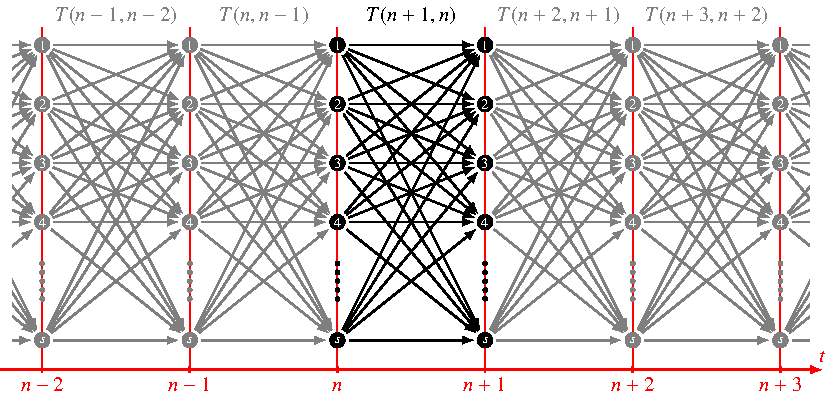
\includegraphics{chapters/80-wahrscheinlichkeit/images/markov.pdf}
\caption{Diskrete Markovkette mit Zuständen $\mathcal{S}=\{1,2,3,\dots,s\}$
und Übergangsmatrizen $T(n+1,n)$.
\label{buch:wahrscheinlichkeit:fig:diskretemarkovkette}}
\end{figure}

Die transienten Übergangswahrscheinlichkeiten zwischen aufeinanderfolgenden
Zeitpunkten stellen jetzt die vollständige Information über die
zeitliche Entwicklung dar
(Abbildung~\ref{buch:wahrscheinlichkeit:fig:diskretemarkovkette}).
Aus der Matrix
\[
T(n+1,n)
=
\begin{pmatrix}
p_{11}(n+1,n) & \dots  & p_{1s}(n+1,n)\\
\vdots        & \ddots & \vdots       \\
p_{11}(n+1,n) & \dots  & p_{1s}(n+1,n)
\end{pmatrix},
\]
auch die $1$-Schritt Übergangswahrscheinlichkeit genannt, kann man jetzt
auch die Matrix der Überganswahrscheinlichkeiten für mehrere Schritte
\[
T(n+m,n)
=
T(n+m,n+m-1)
T(n+m-1,n+m-2)
\dots
T(n+1,n)
\]
mit der Chapman-Komogorov-Formel bestimmen.
Die Markov-Eigenschaft stellt also sicher, dass man nur die 
$1$-Schritt-Übergangswahrscheinlichkeiten kennen muss.

Eine Matrix $T$ kann als Matrix der Übergangswahrscheinlichkeiten
verwendet werden, wenn sie zwei Bedingungen erfüllt:
\begin{enumerate}
\item Die Einträge von $T$ müssen als Wahrscheinlichkeiten interpretiert
werden können, sie müssen also alle zwischen $0$ und $1$ sein:
$0\le t_{ij}\le 1$ für $i,j\in\mathcal{S}$
\item Die Matrix muss alle möglichen Fälle erfassen.
Dazu ist notwendig, dass sich die Wahrscheinlichkeiten aller Übergänge
aus einem Zustand $j$ zu $1$ summieren, also
\[
\sum_{i\in\mathcal{S}} p_{ij} = 1.
\]
Die Summe der Elemente einer Spalte 
\end{enumerate}

\begin{beispiel}
Die Permutationsmatrix einer Permutation $\sigma\in S_n$ 
(Abschnitt~\label{buch:section:permutationsmatrizen})
ist eine Matrix mit Einträgen $0$ und $1$, so dass die erste Bedingung
erfüllt ist.
In jeder Zeile oder Spalte kommt genau eine $1$ vor, so dass auch die
zweite Bedingung erfüllt ist.
Eine Permutationsmatrix beschreibt einen stochastischen Prozess, dessen
Übergänge deterministisch sind.
\end{beispiel}

\subsubsection{Zustandswahrscheinlichkeiten}
% XXX Zustandswahrscheinlichkeit
Die Wahrscheinlichkeit, mit der sich der Prozess zum Zeitpunkt $n$
im Zustand $i\in\mathcal{S}$ befindet, wird
\[
p_i(n)
=
P(X_i=n)
\]
geschrieben, die auch in einem Vektor $p(n)$ zusammengefasst
werden können.
Die Matrix der Übergangswahrscheinlichkeiten erlaubt, die Verteilung
$p(n+1)$ aus der Verteilung $p(n)$ zu berechnen.
Nach dem Satz von der totalen Wahrscheinlichkeit ist nämlich
\[
P(X_{n+1}=x)
=
\sum_{y\in\mathcal{S}} 
P(X_{n+1}=x|X_n=y) P(X_n=y)
\qquad\text{oder}\qquad
p^{(n+1)} = T(n+1,n) p^{(n)}
\]
in Matrixform.
Die Zeitentwicklung kann also durch Multiplikation mit der Übergangsmatrix
berechnet werden.

\subsubsection{Zeitunabhängige Übergangswahrscheinlichkeiten}
% XXX Übergangswahrscheinlichkeit
Besonderes einfach wird die Situation, wenn die Übergangsmatrix $T(n+1,n)$
nicht von der Zeit abhängt.
In diesem Fall ist $T(n+1,n) = T$ für alle $n$.
Eine solche Markov-Kette heisst {\em homogen}.
\index{homogene Markov-Kette}%
Die Mehrschritt-Übergangswahrscheinlichkeiten sind dann gegeben
durch die Matrix-Potenzen $T(n+m,n)=T^m$.
Im Folgenden gehen wir immer von einer homogenen Markov-Kette aus.

\subsubsection{Stationäre Verteilung}
% XXX stationäre Verteilung
Im Beispiel der Google-Matrix erwarten wir intuitiv, dass sich mit
der Zeit eine Verteilung einstellt,  die sich über die Zeit nicht
mehr ändert.
Ein solche Verteilung heisst stationär.

\begin{definition}
Eine Verteilungsvektor $p$ heisst {\em stationär} für die
homogene Markov-Kette mit Übergangsmatrix $T$, wenn $Tp=p$.
\index{stationäre Verteilung}%
\end{definition}

Eine stationäre Verteilung ist offenbar ein Eigenvektor der Matrix
$T$  zum Eigenwert $1$.
Gefunden werden kann er als Lösung des Gleichungssystems $Tp=p$.
Dazu muss die Matrix $T-E$ singulär sein.
Die Summe einer Spalte von $T$ ist aber immer ein, da $E$ in jeder Spalte
genau eine $1$ enthält, ist die Summe der Einträge einer Spalte von
$T-E$ folglich $0$.
Die Summe aller Zeilen von $T-E$ ist also $0$, die Matrix $T-E$ 
ist singulär.
Dies garantiert aber noch nicht, dass alle Einträge in diesem
Eigenvektor auch tatsächlich nichtnegativ sind.
Die Perron-Frobienus-Theorie von
Abschnitt~\ref{buch:section:positive-vektoren-und-matrizen}
beweist, dass sich immer ein Eigenvektor mit nichtnegativen
Einträgen finden lässt.

Es ist aber nicht garantiert, dass eine stationäre Verteilung
auch eindeutig bestimmt ist.
Dieser Fall tritt immer ein, wenn die geometrische Vielfachheit
des Eigenwerts $1$ grösser ist als $1$.
In Abschnitt~\ref{buch:subsection:elementare-eigenschaften}
werden Bedingungen an eine Matrix $T$ untersucht, die garantieren,
dass der Eigenraum zum Eigenvektor $1$ einedeutig bestimmt ist.

\begin{beispiel}
Als Beispiel dafür betrachten wir eine Permutation $\sigma\in S_n$
und die zugehörige Permutationsmatrix $P$,
wie sie in Abschnitt~\label{buch:section:permutationsmatrizen}
beschrieben worden ist.
Wir verwenden die 
Zyklenzerlegung (Abschnitt~\ref{buch:subsection:zyklenzerlegung})
\(
[n] = \{ Z_1, Z_2,\dots \}
\)
der Permutation $\sigma$, ist ist also $\sigma(Z_i) = Z_i$ für alle
Zyklen.

Jede Verteilung $p$, die auf jedem Zyklus konstant ist, ist eine
stationäre Verteilung.
Ist nämlich $i\in Z_k$, dann ist natürlich auch $\sigma(i)\in Z_k$,
und damit ist $p_{\sigma(i)}=p_i$.

Für jede Wahl von nichtnegativen Zahlen $z_i$ für $i=1,\dots,k$
mit der Eigenschaft $z_1+\dots+z_k=1$ kann man eine stationäre
Verteilung $p(z)$ konstruieren, indem man
\[
p_i(z)
=
\frac{z_i}{|Z_r|}
\qquad\text{wenn}\quad i\in Z_r
\]
setzt.
Die Konstruktion stellt sicher, dass sich die Komponenten zu $1$
summieren.
Wir können aus dem Beispiel auch ableiten, dass die geometrische
Vielfachheit des Eigenvektors $1$ mindestens so gross ist wie die
Anzahl der Zyklen der Permutation $\sigma$.
\end{beispiel}

\subsubsection{Irreduzible Markov-Ketten}
Die Zyklen-Zerlegung einer Permutation bilden voneinander isolierte
Mengen von Zuständen, es gibt keine Möglichkeit eines Übergangs zu
einem anderen Zyklus.
Die Zyklen können daher unabhängig voneinander studiert werden.
Diese Idee kann auf allgemeine Markov-Ketten verallgemeinert werden.

\begin{definition}
Zwei Zustände $i,j\in\mathcal{S}$ kommunizieren, wenn die
Übergangswahrscheinlichkeiten $T_{ij}(n) \ne 0$ und $T_{ij}(n)\ne 0$ sind
für $n$ gross genug.
\end{definition}

Die Zustände, die zu verschiedenen Zyklen einer Permutation gehören,
kommunizieren nicht.
Gerade deshalb waren auch die verschiedenen stationären Verteilungen
möglich.
Eine eindeutige stationäre Verteilung können wir also nur erwarten,
wenn alle Zustände miteinander kommunizieren.

% XXX irreduzible Markov-Ketten
\begin{definition}
Eine homogene Markov-Kette heisst {\em irreduzibel}, alle Zustände miteinander
kommunizieren.
\index{irreduzible Markov-Kette}
\end{definition}

\begin{figure}
\centering
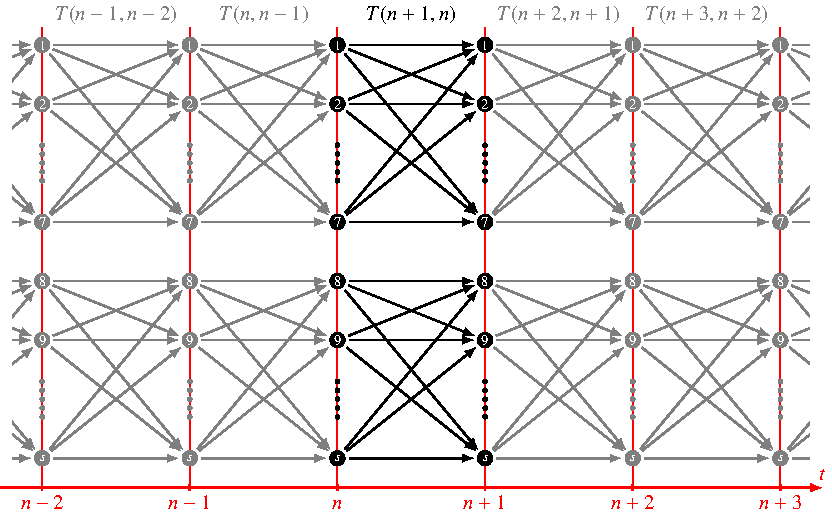
\includegraphics{chapters/80-wahrscheinlichkeit/images/markov2.pdf}
\caption{Diese Markov-Kette zerfällt in verschiedene irreduzible
Markov-Ketten, dere Zustandsmengen nicht miteinander kommunizieren.
Solche Markov-Ketten können unabhängig voneinander studiert werden.
\label{buch:wahrscheinlichkeit:fig:markovzerfall}}
\end{figure}

Die Bedingung der Irreduzibilität ist gleichbedeutend damit,
dass für genügend grosses $n$ alle Matrixelemente von $T^n$ positiv sind.
Solche Matrizen nennt man positiv, 
in Abschnitt~\ref{buch:section:positive-vektoren-und-matrizen}
wird gezeigt, dass positive Matrizen immer eine eindeutige
stationäre Verteilung haben.
In Abbildung~\ref{buch:wahrscheinlichkeit:fig:markovzerfall}
ist eine reduzible Markov-Kette dargestellt, die Zustandsmenge
zerfällt in zwei Teilmengen von Zuständen, die nicht miteinander
kommunizieren.
Ein irreduzible Markov-Kette liegt vor, wenn sich ähnlich wie
in Abbildung~\ref{buch:wahrscheinlichkeit:fig:diskretemarkovkette}
jeder Zustand von jedem anderen aus erreichen lässt.

Wenn sich der Vektorraum $\mathbb{R}^n$ in zwei unter $T$ invariante
Unterräme zerlegen lässt, dann hat nach Wahl von Basen in den Unterräumen
die Matrix $T$ die Form
\[
\left(
\begin{array}{c|c}
T_1&0\\
\hline
0&T_2
\end{array}
\right).
\]
Insbesondere kann man stationäre Verteilungen von $T_1$ und $T_2$ 
unabhängig voneinander suchen.
Ist $p_i$ eine stationäre Verteilung von $T_i$, dann ist
\[
T
\left(
\begin{array}{c}
g_1p_1\\
\hline g_2p_2
\end{array}
\right)
=
\left(
\begin{array}{c}
g_1T_1p_1\\
\hline
g_2T_2p_2
\end{array}
\right)
=
\left(
\begin{array}{c}
g_1p_1\\
\hline
g_2p_2
\end{array}
\right),\qquad
\text{ für $g_i\in\mathbb{R}$.}
\]
Durch Wahl der Gewichte $g_i\ge 0$ mit $g_1+g_2=1$ lassen sich so
die stationären Verteilungen für $T$ aus den stationären Verteilungen
der $T_i$ ermitteln.
Das Problem, die stationären Verteilungen von $T$ zu finden, ist
auf die Untermatrizen $T_i$ reduziert worden.

\subsubsection{Die konvexe Menge der stationären Verteilungen}
\begin{figure}
\centering
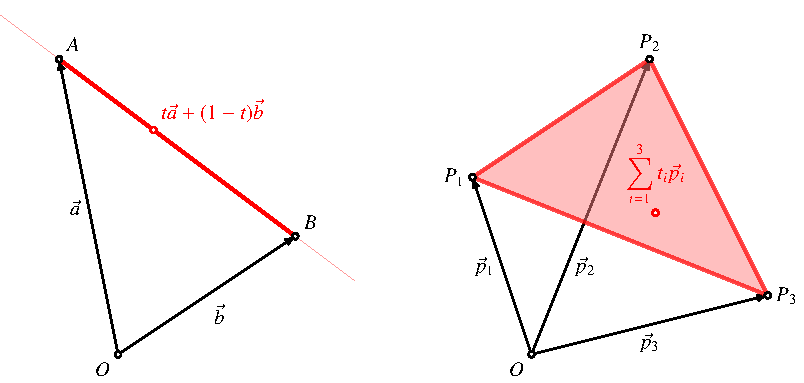
\includegraphics{chapters/80-wahrscheinlichkeit/images/konvex.pdf}
\caption{Die Konvexe Kombination von Vektoren $\vec{p}_1,\dots,\vec{p}_n$ ist
eine Summe der Form $\sum_{i=1}^n t_i\vec{p}_i$ wobei die $t_i\ge 0$
sind mit $\sum_{i=1}^nt_i=1$.
Für zwei Punkte bilden die konvexen Kombinationen die Verbindungsstrecke
zwischen den Punkten, für drei Punkte in drei Dimensionen spannen die
konvexen Kombinationen ein Dreieck auf.
\label{buch:wahrscheinlichkeit:fig:konvex}}
\end{figure}
Die stationären Verteilungen
\[
\operatorname{Stat}(T)
=
\{
p\in\mathbb R_+^n\;|\; \text{$Tp=p $ und $\|p\|_1=1$}
\}
\]
bilden was man eine konvexe Menge nennt.
Sind nämlich $p$ und $q$ stationäre Verteilungen, dann gilt zunächst
$Tp=p$ und $Tq=q$.
Wegen der Linearität gilt aber auch $T(tp+(1-t)q)=tTp + (1-t)Tq
=tp+(1-t)q$.
Jede Verteilung auf der ``Verbindungsstrecke'' zwischen den beiden
Verteilungen ist auch wieder stationär.

\begin{definition}
Eine {\em konvexe Kombination} von Vektoren $v_1,\dots,v_k\in\mathbb{R^n}$
ist ein Vektor der Form
\[
v=t_1v_1+\dots + t_kv_k
\qquad\text{mit}\quad
t_i\ge 0\;\text{und}\;
t_1+\dots+t_n = 1.
\]
\index{konvexe Kombination}%
Eine Teilmenge $M\subset \mathbb{R}^n$ heisst konvex, wenn zu
zwei Vektoren $x,y\in M$ auch jede konvexe Kombination von $x$ und $y$
wieder in $M$ ist.
\index{konvex}%
\end{definition}

Die konvexen Kombinationen der Vektoren sind Linearkombination
mit nichtnegativen Koeffizienten. Sie bilden im Allgemeinen
einen $(k-1)$-Simplex in $\mathbb{R}^n$.
Für zwei Punkte $x$ und $y$ bilden die konvexen Kombination
$tx+(1-t)y$ für $t\in[0,1]$ die Verbindungsstrecke der beiden
Vektoren.
Eine Menge ist also konvex, wenn sie mit zwei Punkten immer auch
ihre Verbindungsstrecke enthält
% XXX Bild für Konvexe Menge



% XXX Grenzverteilung
\subsubsection{Grenzverteilung}
Im Beispiel der Google-Matrix wurde ein iterativer Algorithmus
zur Berechnung des Pagerank verwendet.
Es stellt sich daher die Frage, ob diese Methode für andere homogene
Markov-Ketten auch funkioniert.
Man beginnt also mit einer beliebigen Verteilung $p(0)$ und wendet
die Übergangsmatrix $T$ wiederholt an.
Es entsteht somit eine Folge $p(n) = T^np(0)$.

\begin{definition}
Falls die Folge $p(n) = T^np(0)$ konvergiert, heisst der Grenzwert
\[
p(\infty) = \lim_{n\to\infty} p(n)
\]
eine {\em Grenzverteilung} von $T$.
\index{Grenzverteilung}%
\end{definition}

Falls eine Grenzverteilung existiert, dann ist sie eine stationäre
Verteilung.
Für eine stationäre Verteilung $p(0)$ ist die Folge $p(n)$ eine
konstante Folge, sie konvergiert also gegen $p(0)$.
Stationäre Verteilungen sind also automatisch Grenzverteilungen.
Falls der Raum der stationären Verteilungen mehrdimensional sind,
dann ist auch die Grenzverteilung nicht eindeutig bestimmt, selbst
wenn sie existiert.
Aber nicht einmal die Existenz einer Grenzverteilung ist garantiert,
wie das folgende Beispiel zeigt.

\begin{beispiel}
Sei $T$ die Permutationsmatrix der zyklischen Verteilung von drei
Elementen in $S_3$, also die Matrix
\[
T=\begin{pmatrix}
0&0&1\\
1&0&0\\
0&1&0
\end{pmatrix}.
\]
Die konstante Verteilung $\frac13U$ ist offensichtlich eine
stationäre Verteilung.
In Abschnitt~\ref{buch:section:positive-vektoren-und-matrizen}
wird gezeigt, dass es die einzige ist.
Sei jetzt $p(0)$ eine beliebiger Vektor in $\mathbb{R}^3$ mit
nichtnegativen Einträgen, die sich zu $1$ summieren.
Dann bilden die Vektoren $p(n)=T^np(0)$ einen Dreierzyklus
\begin{align*}
p(0)&=p(3)=p(6)=\dots =\begin{pmatrix}p_1(0)\\p_2(0)\\p_3(0)\end{pmatrix},
\\
p(1)&=p(4)=p(7)=\dots =\begin{pmatrix}p_2(0)\\p_3(0)\\p_1(0)\end{pmatrix},
\\
p(2)&=p(5)=p(8)=\dots =\begin{pmatrix}p_3(0)\\p_1(0)\\p_2(0)\end{pmatrix}.
\end{align*}
Die Folge $p(n)$ kann also nur dann konvergieren, wenn die drei
Komponenten gleich sind.
\end{beispiel}

\subsubsection{Erwartungswert und Varianz}
% XXX Erwartungswert und Varianz für eine Grenzverteilung
Wenn sich im Laufe der Zeit eine Grenzverteilung einstellen soll, dann
muss es auch möglich sein, Erwartungswert und Varianz dieser Verteilung
zu berechnen.
Dazu muss jedem Zustand ein Zahlenwert zugeordnet werden.
Sei also
\(
g: \mathcal{S}\to R
\)
eine Funktion, die einem Zustand eine reelle Zahl zuordnet.
Aus der Zufallsvariable $X_n$ des Zustands zur Zeit $n$ wird daraus
die Zufallsvariable $Y_n=g(X_n)$ des Wertes zur Zeit $n$.
Die Abbildung $g$ kann auch als Vektor mit der Komponenten $g_i$ 
für $i\in\mathcal{S}$ betrachtet werden, wir verwenden für diesen
Vektor wieder die Schreibweise $g$.

Für die Verteilung $p(n)$ kann man jetzt auch Erwartungswert und
Varianz berechnen.
Der Erwartungswert ist
\[
E(Y)
=
\sum_{i\in\mathcal{S}} g_i p_i(n)
=
g^t p(n).
\]
Für die Varianz muss $g_i$ durch $g_i^2$ ersetzt werden.
Dies kann am einfachsten mit dem Hadamard-Produkt geschrieben werden:
\begin{align*}
E(Y^2)
&=
\sum_{i\in\mathcal{S}} g_i p_i(n)
=
(g\odot g)^t p(n)
\\
E(Y^k)
&=
(g^{\odot k})^t p(n),
\end{align*}
wobei wir die Hadamard-Potenz $A^{\odot k}$ einer Matrix $A$ rekursiv
durch
\[
A^{\odot 0}=E
\qquad\text{und}\qquad
A^{\odot k} = A\odot A^{\odot (k-1)}
\]
definieren.

\subsubsection{Erwartungswert von Werten auf Übergängen}
% XXX Erwartungswert für Zufallsvariablen, die von den Übergängen abhängen
In Abschnitt~\ref{buch:section:paradoxon-von-parrondo} wird ein Spiel
vorgestellt, in dem der Gewinn davon abhängt, welcher Übergang stattfindet,
nicht welcher Zustand erreicht wird.
Es git daher eine Matrix $G$ von Gewinnen, der Eintrag $g_{ij}$ ist
der Gewinn, der bei einem Übergang von Zustand $j$ in den Zustand $i$
ausgezahlt wird.
Mit dieser Matrix lassen sich jetzt viele verschiedene Fragen beantworten:

\begin{frage}
\label{buch:wahrscheinlichkeit:frage1}
Mit welchem Gewinn kann man in Runde $n$ des Spiels rechnen,
wenn $p(n-1)$ die Verteilung zur Zeit $n-1$ ist?
\end{frage}

Der Erwartungswert ist
\begin{align*}
E(Y)
&=
\sum_{i,j\in\mathcal{S}}
g_{ji} t_{ji} p_i(n-1)
\intertext{oder in Matrixform}
&=
U^t
(G\odot T)
p(n-1).
\end{align*}

\begin{frage}
Mit welchen Gewinnen kann man rechnen, wenn der Prozess sich zu Beginn 
einer Spielrunde im Zustand $i$ befindet?
\end{frage}

Dies ist der Spezialfall der Frage~\ref{buch:wahrscheinlichkeit:frage1}
für die Verteilung $p_j(n-1) = \delta_{ij}$.
Der Erwartungswert ist die Summe der Spalte $j$ der Matrix $G\odot T$.
Man kann das Produkt $U^t(G\odot T)$ also auch als eine Zeilenvektor
von Gewinnerwartungen unter der Vorbedingung $X_{n-1}=j$ betrachten.
\[
\begin{pmatrix}
E(Y|X_{n-1}=1)
&\dots&
E(Y|X_{n-1}=n)
\end{pmatrix}
=
U^t (G\odot T).
\]
Indem man $G$ durch $G^{\odot k}$ ersetzt, kann man beliebige höhere
Momente berechnen.

\subsection{Absorbierende Zustände}
% XXX Definition
Eine Grenzverteilung beschreibt die relative Häufigkeit, mit der
der Prozess in den verschiedenen Zuständen vorbeikommt.
In einem Spiel, in dem der Spieler ruiniert werden kann, gibt es
aus dem Ruin-Zustand keinen Weg zurück.
Der Spieler bleibt in diesem Zustand.

\begin{definition}
Ein Zustand $i$ einer homogenen Markov-Kette mit Übergangsmatrix $T$
heisst {\em absorbierend}, wenn $T_{ii}=1$ ist.
\index{absorbierender Zustand}%
Eine Markov-Kette mit mindestens einem absorbierenden Zustand heisst
{\em absorbierende Markov-Kette}.
\index{absorbierende Markov-Kette}%
Nicht absorbierende Zustände heissen {\em transient}
\index{transienter Zustand}%
\end{definition}

\begin{figure}
\centering
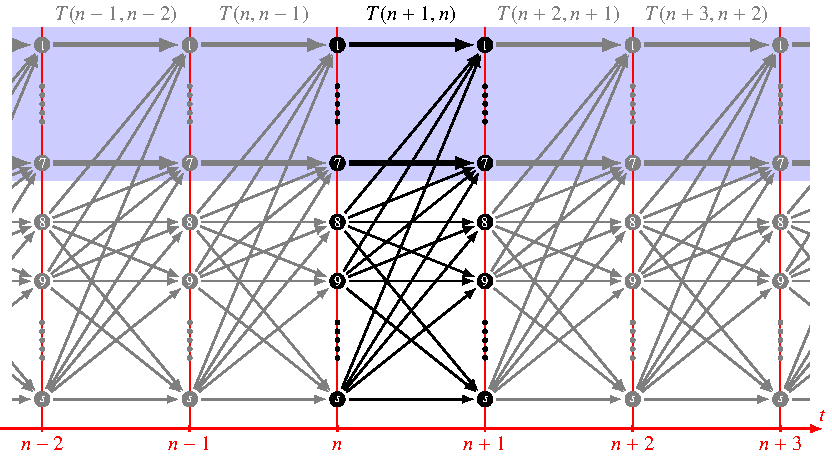
\includegraphics{chapters/80-wahrscheinlichkeit/images/markov3.pdf}
\caption{Markov-Kette mit absorbierenden Zuständen (blau hinterlegt).
Erreicht die Markov-Kette einen absorbierenden Zustand, dann verbleibt
sie für alle zukünftigen Zustände in diesem Zustand.
\label{buch:wahrscheinlichkeit:fig:abs}}
\end{figure}

Eine Markov-Kette kann mehrere absorbierende Zustände haben, wie in
Abbildung~\ref{buch:wahrscheinlichkeit:fig:abs} dargestellt.
Indem man die absorbierenden Zustände zuerst auflistet, bekommt die 
Übergangsmatrix die Form
\[
T=
\left(
\begin{array}{c|c}
E&R\\
\hline
0&Q
\end{array}
\right).
\]
Die Matrix $R$ beschreibt die Wahrscheinlichkeiten, mit denen man
ausgehend von einem transienten Zustand
in einem bestimmten absorbierenden Zustand landet.
Die Matrix $Q$ beschreibt die Übergänge, bevor dies passiert.
Die Potenzen von $T$ sind
\[
T^2
=
\left(
\begin{array}{c|c}
E&R+RQ \\
\hline
0&Q^2
\end{array}
\right),
\quad
T^3
=
\left(
\begin{array}{c|c}
E&R+RQ+RQ^2 \\
\hline
0&Q^3
\end{array}
\right),
\;
\dots,
\;
T^k
=
\left(
\begin{array}{c|c}
E&\displaystyle R\sum_{l=0}^{k-1} Q^l \\
\hline
0&Q^k
\end{array}
\right).
\]
Da man früher oder später in einem absorbierenden Zustand landet,
muss $\lim_{k\to\infty} Q^k=0$ sein.
Die Summe in der rechten oberen Teilmatrix kann man als geometrische
Reihe summieren, man erhält die Matrix
\[
\sum_{l=0}^{k-1} Q^l = (E-Q)^{-1}(E-Q^k),
\]
die für $k\to\infty$ gegen
\[
N
=
\lim_{k\to\infty} \sum_{l=0}^{k-1} Q^l
=
(E-Q)^{-1}
\]
konvergiert.
Die Matrix $N$ heisst die {\em Fundamentalmatrix} der absorbierenden
Markov-Kette.
\index{Fundamental-Matrix}%

\subsubsection{Absorbtionszeit}
% XXX Absorptionszeit
Wie lange dauert es im Mittel, bis der Prozess in einem
Absorptionszustand $i$ stecken bleibt?
Die Fundamentalmatrix $N$ der Markov-Kette beantwortet diese
Frage.
Wenn der Prozess genau im Schritt $k$ zum ersten Mal Zustand $i$
ankommt, dann ist $E(k)$ die mittlere Wartezeit.
Der Prozess verbringt also zunächst $k-1$ Schritte in transienten
Zuständen, bevor er in einen absorbierenden Zustand wechselt.

Wir brauchen die Wahrscheinlichkeit für einen Entwicklung des Zustandes
ausgehend vom Zustand $j$, die nach $k-1$ Schritten im Zustand $l$
landet, von wo er in den absorbierenden Zustand wechselt.
Diese Wahrscheinlichkeit ist
\[
P(X_k = i\wedge X_{k-1} = l \wedge X_0=j)
=
\sum_{i_1,\dots,i_{k-2}}
r_{il} q_{li_{k-2}} q_{i_{k-2}i_{k-3}}\dots q_{i_2i_1} q_{i_1j}
\]
Von den Pfaden, die zur Zeit $k-1$ im Zustand $l$ ankommen gibt es
aber auch einige, die nicht absorbiert werden.
Für die Berechnung der Wartezeit möchten wir nur die Wahrscheinlichkeit
innerhalb der Menge der Pfade, die auch tatsächlich absorbiert werden,
das ist die bedingte Wahrscheinlichkeit
\begin{equation}
\begin{aligned}
P(X_k = i\wedge X_{k-1} = l \wedge X_0=j|X_k=i)
&=
\frac{
P(X_k = i\wedge X_{k-1} = l \wedge X_0=j)
}{
P(X_k=i)
}
\\
&=
\sum_{i_1,\dots,i_{k-2}}
q_{li_{k-2}} q_{i_{k-2}i_{k-3}}\dots q_{i_2i_1} q_{i_1j}.
\end{aligned}
\label{buch:wahrscheinlichkeit:eqn:ankunftswahrscheinlichkeit}
\end{equation}
Auf der rechten Seite steht das Matrixelement $(l,j)$ von $Q^{k-1}$.

% XXX Differenz 

Für die Berechnung der erwarteten Zeit ist müssen wir die
Wahrscheinlichkeit mit $k$ multiplizieren und summieren:
\begin{align}
E(k)
&=
\sum_{k=0}^\infty
k(
q^{(k)}_{lj} 
-
q^{(k-1)}_{lj} 
)
\notag
\\
&=
\dots
+
(k+1)(
q^{(k)}_{lj} 
-
q^{(k+1)}_{lj} 
)
+
k(
q^{(k-1)}_{lj} 
-
q^{(k)}_{lj} 
)
+
\dots
\label{buch:wahrscheinlichkeit:eqn:telescope}
\\
&=
\dots
+
q^{(k-1)}_{lj}
+
\dots
=
\sum_{k} q^{(k)}_{lj}.
\notag
\end{align}
In zwei benachbarten Termen in 
\eqref{buch:wahrscheinlichkeit:eqn:telescope}
heben sich die Summanden $kq^{(k)}_{lj}$ weg, man spricht von
einer teleskopischen Reihe.
Die verbleibenden Terme sind genau die Matrixelemente der Fundamentalmatrix $N$.
Die Fundamentalmatrix enthält also im Eintrag $(l,j)$ die Wartezeit
bis zur Absorption über den Zustand $l$.

\subsubsection{Wartezeit}
% XXX Mittlere Zeit bis zu einem bestimmten Zustand
Die mittlere Wartezeit bis zum Erreichen eines Zustands kann mit der
Theorie zur Berechnung der Absorptionszeit berechnet werden.
Dazu modifiziert man den Prozess dahingehend, dass der Zielzustand
ein absorbierender Zustand wird.
Der Einfachheit halber gehen wir davon aus, dass der Zustand $1$ 
der Zielzustand ist.
Wir ersetzen die Übergangsmatrix $T$ durch die Matrix
\[
\tilde{T}
=
\left(
\begin{array}{c|ccc}
1     &t_{12}&\dots &t_{1n}\\
\hline
0     &t_{22}&\dots &t_{2n}\\
\vdots&\dots &\ddots&\vdots\\
0     &t_{n2}&\dots &t_{nn}
\end{array}\right).
\]
$\tilde{T}$ hat den Zustand $1$ als absorbierenden Zustand.
Die $Q$ und $R$ sind
\[
\tilde{R}
=
\begin{pmatrix}t_{12}&\dots&t_{1n}\end{pmatrix},
\quad
\tilde{Q}
=
\begin{pmatrix}
t_{22}&\dots &t_{2n}\\
\vdots&\ddots&\vdots\\
t_{n2}&\dots &t_{nn}
\end{pmatrix}.
\]
Die Wartezeit bis zum Erreichen des Zustands $i$ ausgehend von einem
Zustand $n$ kann jetzt aus der Absorbtionszeit der Markov-Kette
im Zustand $1$ mit Hilfe der Fundamentalmatrix
\[
\tilde{N} 
=
(E-\tilde{Q})^{-1}
\]
berechnet werden.



%
% positiv.tex
%
% (c) 2021 Prof Dr Andreas Müller, OST Ostschweizer Fachhochschule
%
\documentclass[tikz]{standalone}
\usepackage{times}
\usepackage{amsmath}
\usepackage{txfonts}
\usepackage[utf8]{inputenc}
\usepackage{graphics}
\usetikzlibrary{arrows,intersections,math}
\usepackage{ifthen}
\begin{document}

\newboolean{showgrid}
\setboolean{showgrid}{false}
\def\breite{7}
\def\hoehe{4}

\begin{tikzpicture}[>=latex,thick]

% Povray Bild
\node at (0,0) {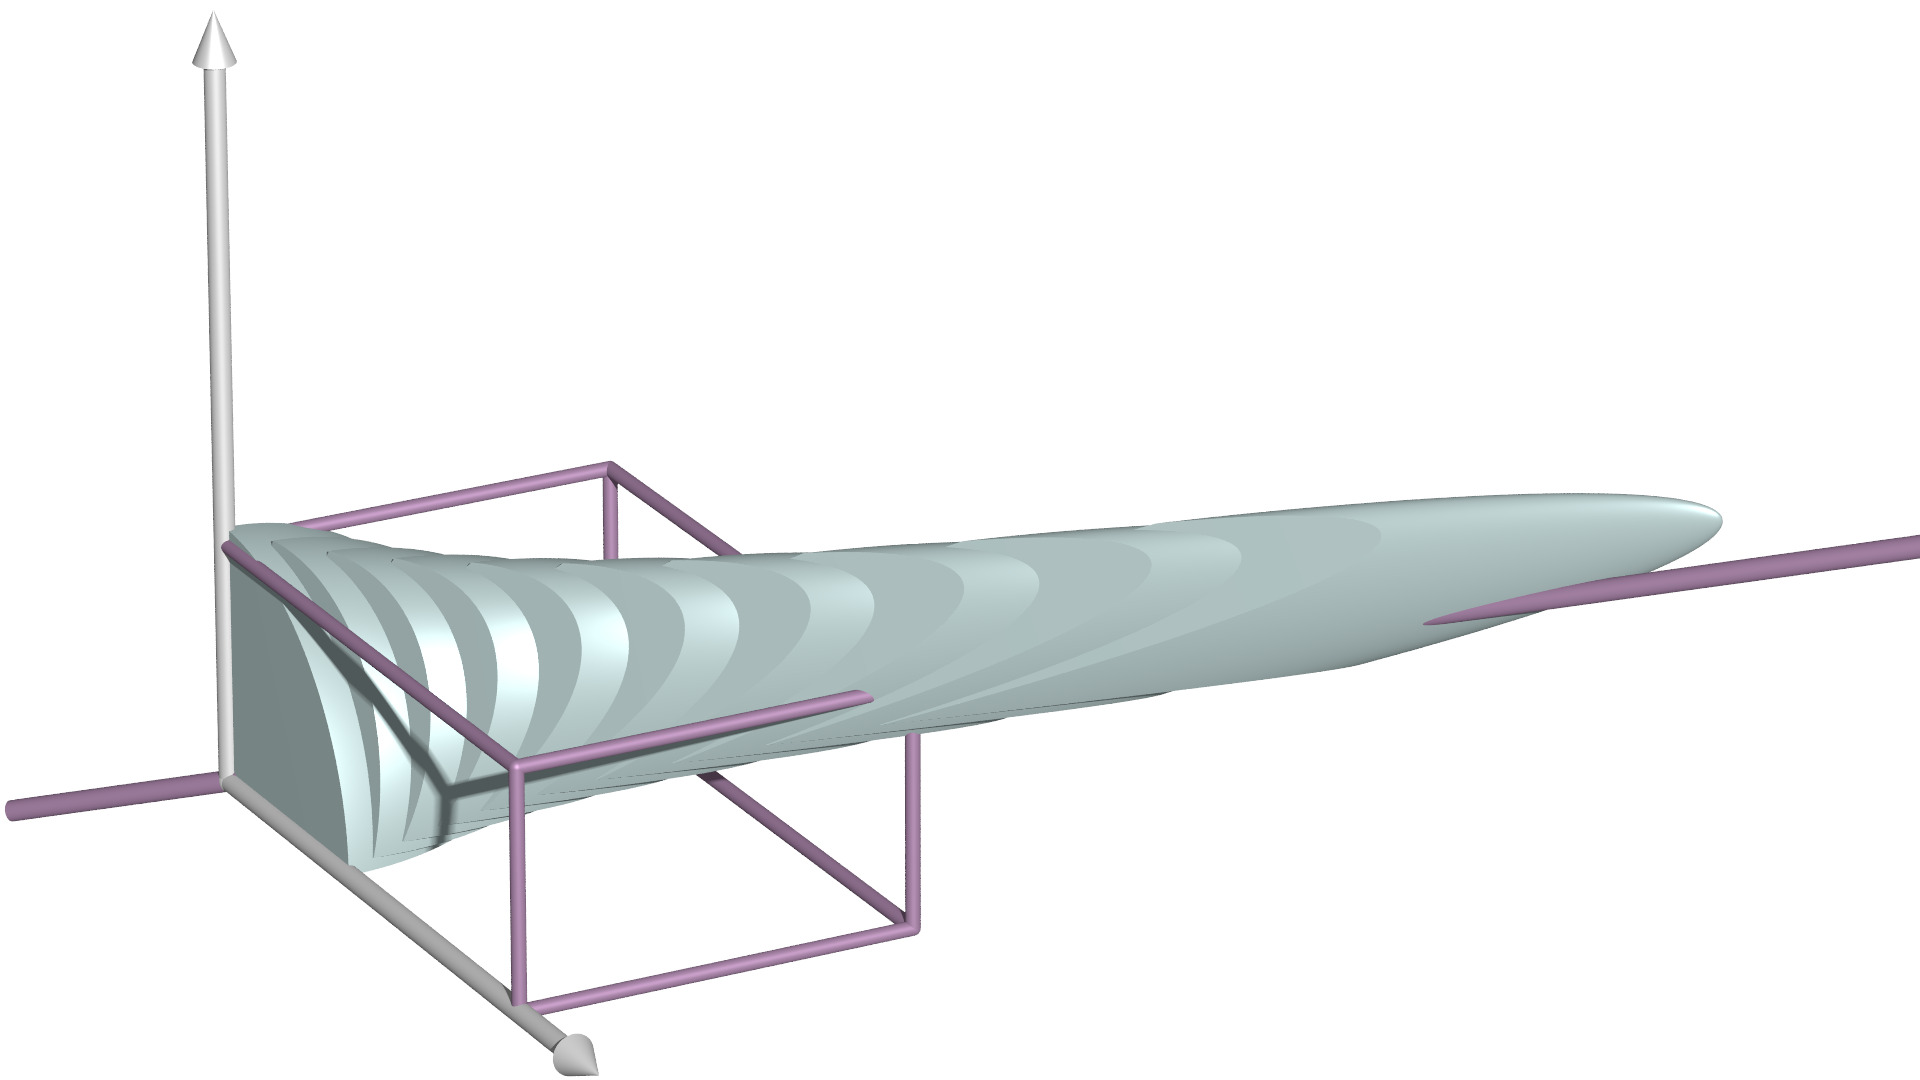
\includegraphics[width=14cm]{positiv.jpg}};

% Gitter
\ifthenelse{\boolean{showgrid}}{
\draw[step=0.1,line width=0.1pt] (-\breite,-\hoehe) grid (\breite, \hoehe);
\draw[step=0.5,line width=0.4pt] (-\breite,-\hoehe) grid (\breite, \hoehe);
\draw                            (-\breite,-\hoehe) grid (\breite, \hoehe);
\fill (0,0) circle[radius=0.05];
}{}

\node at (-2.6,-3.8) [right] {$x_1$};
\node at (-5.4,3.8) [right] {$x_3$};

\node[color=red] at (-4.5,-1.3) {$0$};
\node[color=red] at (-4.15,-1.25) {$1$};
\node[color=red] at (-3.75,-0.90) {$2$};
\node[color=red] at (-3.22,-0.80) {$3$};
\node[color=red] at (-2.6,-0.70) {$4$};
\node[color=red] at (-1.8,-0.60) {$5$};
\node[color=red] at (-0.9,-0.50) {$6$};
\node[color=red] at (0.2,-0.40) {$7$};
\node[color=red] at (1.6,-0.20) {$8$};
\node[color=red] at (4.0,0.10) {$9$};

\end{tikzpicture}

\end{document}


%
% parrondo.tex -- Anwendung: analyse von Parrondos Paradoxon
%
% (c) 2020 Prof Dr Andreas Müller, Hochschule Rapperswil
%
\section{Das Paradoxon von Parrondo
\label{buch:section:paradoxon-von-parrondo}}
\rhead{Das Paradoxon von Parrondo}
Das Paradoxon von Parrondo ist ein der Intuition widersprechendes
Beispiel für eine Kombination von Spielen mit negativer Gewinnerwartung,
deren Kombination zu einem Spiel mit positiver Gewinnerwartung führt.
Die Theorie der Markov-Ketten und der zugehörigen Matrizen ermöglicht
eine sehr einfache Analyse.

%
% Parrondo Teilspiele
%
\subsection{Die beiden Teilspiele
\label{buch:subsection:teilspiele}}

\subsubsection{Das Spiel $A$}
Das Spiel $A$ besteht darin, eine Münze zu werfen.
Je nach Ausgang gewinnt oder verliert der Spieler eine Einheit.
Sei $X$ die Zufallsvariable, die den gewonnen Betrag beschreibt.
Für eine faire Münze ist die Gewinnerwartung in diesem Spiel natürlich
$E(X)=0$.
Wenn die Wahrscheinlichkeit für einen Gewinn $\frac12+e$ ist, dann muss
die Wahrscheinlichkeit für einen Verlust $\frac12-e$ sein, und die 
Gewinnerwartung ist
\(
E(X)
=
1\cdot P(X=1) + (-1)\cdot P(X=-1)
=
\frac12+e + (-1)\biggl(\frac12-e\biggr)
=
2e.
\)
Die Gewinnerwartung ist also genau dann negativ, wenn $e<0$ ist.

\subsubsection{Das Spiel $B$}
Das zweite Spiel $B$ ist etwas komplizierter, da der Spielablauf vom 
aktuellen Kapital $K$ des Spielers abhängt.
Wieder gewinnt oder verliert der Spieler eine Einheit,
die Gewinnwahrscheinlichkeit hängt aber vom Dreierrest des Kapitals ab.
Sei $Y$ die Zufallsvariable, die den Gewinn beschreibt.
Ist $K$ durch drei teilbar, ist die Gewinnwahrscheinlichkeit $\frac1{10}$,
andernfalls ist sie $\frac34$.
Formell ist
\begin{equation}
\begin{aligned}
P(Y=1|\text{$K$ durch $3$ teilbar}) &=  \frac{1}{10}
\\
P(Y=1|\text{$K$ nicht durch $3$ teilbar}) &= \frac{3}{4}
\end{aligned}
\label{buch:wahrscheinlichkeit:eqn:Bwahrscheinlichkeiten}
\end{equation}
Insbesondere ist die Wahrscheinlichkeit für einen Gewinn in zwei der
Fälle recht gross, in einem Fall aber sehr klein.

\subsubsection{Übergangsmatrix im Spiel $B$}
\begin{figure}
\centering
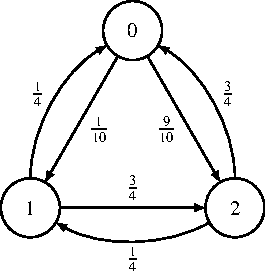
\includegraphics{chapters/80-wahrscheinlichkeit/images/spielB.pdf}
\caption{Zustandsdiagramm für das Spiel $B$, Zustände sind die
Dreierreste des Kapitals.
\label{buch:wahrscheinlichkeit:fig:spielB}}
\end{figure}%
Für den Verlauf des Spiels spielt nur der Dreierrest des Kapitals
eine Rolle.
Es gibt daher drei mögliche Zustände $0$, $1$ und $2$.
In einem Spielzug finde ein Übergang in einen anderen Zustand
statt, der Eintrag $b_{ij}$ ist die Wahrscheinlichkeit
\[
b_{ij}
=
P(K\equiv i|K\equiv j),
\]
dass ein Übergang vom Zustand $j$ in den Zustand $i$ stattfindet.
Die Matrix ist
\[
B=
\begin{pmatrix}
0          &\frac14 &\frac34\\
\frac1{10} &0       &\frac14\\
\frac9{10} &\frac34 &0
\end{pmatrix}.
\]

\subsubsection{Gewinnerwartung in einem Einzelspiel $B$}
Die Gewinnerwartung einer einzelnen Runde des Spiels $B$ hängt natürlich
ebenfalls vom Ausgangskapital ab.
Mit den Wahrscheinlichkeiten von 
\eqref{buch:wahrscheinlichkeit:eqn:Bwahrscheinlichkeiten}
findet man die Gewinnerwartung
\begin{equation}
\begin{aligned}
E(Y| \text{$K$ durch $3$ teilbar})
&=
1\cdot P(Y=1|K\equiv 0\mod 3)
+
(-1)\cdot P(Y=-1|K\equiv 0\mod 3)
\\
&=
\frac1{10}
-
\frac{9}{10}
=
-\frac{8}{10}
\\
E(Y| \text{$K$ nicht durch $3$ teilbar})
&=
1\cdot P(Y=1|K\not\equiv 0\mod 3)
+
(-1)\cdot P(Y=-1|K\not\equiv 0\mod 3)
\\
&=
\frac34-\frac14
=
\frac12.
\end{aligned}
\label{buch:wahrscheinlichkeit:eqn:Berwartungen}
\end{equation}
Falls $K$ durch drei teilbar ist, muss der Spieler
also mit einem grossen Verlust rechnen, andernfalls mit einem
moderaten Gewinn.

Ohne weiteres Wissen über das Anfangskapital ist es zulässig anzunehmen,
dass die drei möglichen Reste die gleiche Wahrscheinlichkeit haben.
Die Gewinnerwartung in diesem Fall ist dann
\begin{align}
E(Y)
&=
E(Y|\text{$K$ durch $3$ teilbar}) \cdot \frac13
+
E(Y|\text{$K$ nicht durch $3$ teilbar}) \cdot \frac23
\notag
\\
&=
-\frac{8}{10}\cdot\frac{1}{3}
+
\frac{1}{2}\cdot\frac{2}{3}
=
-\frac{8}{30}+\frac{10}{30}
=
\frac{2}{30}
=
\frac{1}{15}.
\label{buch:wahrscheinlichkeit:eqn:Beinzelerwartung}
\end{align}
Unter der Annahme, dass alle Reste die gleiche Wahrscheinlichkeit haben,
ist das Spiel also ein Gewinnspiel.

Die Berechnung der Gewinnerwartung in einem Einzelspiel kann man 
wie folgt formalisieren.
Die Matrix $B$ gibt die Übergangswahrscheinlichkeiten zwischen
verschiedenen Zuständen.
Die Matrix 
\[
G=\begin{pmatrix}
 0&-1& 1\\
 1& 0&-1\\
-1& 1& 0
\end{pmatrix}
\]
gibt die Gewinne an, die bei einem Übergang anfallen.
Die Matrixelemente $g_{ij}b_{ij}$ des Hadamard-Produktes 
$G\odot B$
von $G$ mit $B$ enthält in den Spalten die Gewinnerwartungen
für die einzelnen Übergänge aus einem Zustand.
Die Summe der Elemente der Spalte $j$ enthält die Gewinnerwartung
\[
E(Y|K\equiv j)
=
\sum_{i=0}^2 g_{ij}b_{ij}
\]
für einen Übergang aus dem Zustand $j$.
Man kann dies auch als einen Zeilenvektor schreiben, der durch Multiplikation
der Matrix $G\odot B$ mit dem Zeilenvektor
$U^t=\begin{pmatrix}1&1&1\end{pmatrix}$
entsteht:
\[
\begin{pmatrix}
E(Y|K\equiv 0)&
E(Y|K\equiv 1)&
E(Y|K\equiv 2)
\end{pmatrix}
=
U^t
G\odot B.
\]
Die Gewinnerwartung ist dann das Produkt
\[
E(Y)
=
\sum_{i=0}^2
E(Y|K\equiv i) p_i
=
U^t
(G\odot B)p.
\]
Tatsächlich ist
\[
G\odot B
=
\begin{pmatrix}
 0          &-\frac14 & \frac34\\
 \frac1{10} & 0       &-\frac14\\
-\frac9{10} & \frac34 & 0
\end{pmatrix}
\quad\text{und}\quad
U^t G\odot B
=
\begin{pmatrix}-\frac{8}{10}&\frac12&\frac12\end{pmatrix}.
\]
Dies stimmt mit den Erwartungswerten in 
\eqref{buch:wahrscheinlichkeit:eqn:Berwartungen}
überein.
Die gesamte Geinnerwartung ist dann
\begin{equation}
(G\odot B)
\begin{pmatrix}\frac13\\\frac13\\\frac13\end{pmatrix}
=
\begin{pmatrix}-\frac{8}{10}&\frac12&\frac12\end{pmatrix}
\frac13U
=
\frac13\biggl(-\frac{8}{10}+\frac12+\frac12\biggr)
=
\frac13\cdot\frac{2}{10}
=
\frac{1}{15},
\label{buch:wahrscheinlichkeit:eqn:BodotEinzelerwartung}
\end{equation}
dies stimmt mit \eqref{buch:wahrscheinlichkeit:eqn:Beinzelerwartung}
überrein.

\subsubsection{Das wiederholte Spiel $B$}
Natürlich spielt man das Spiel nicht nur einmal, sondern man wiederholt es.
Es ist verlockend anzunehmen, dass die Dreierreste $0$, $1$ und $2$ des
Kapitals immer noch gleich wahrscheinlich sind.
Dies braucht jedoch nicht so zu sein.
Wir prüfen die Hypothese daher, indem wir die Wahrscheinlichkeit
für die verschiedenen Dreierreste des Kapitals in einem interierten
Spiels ausrechnen.

Das Spiel kennt die Dreierreste als die drei für das Spiel ausschlaggebenden
Zuständen.
Das Zustandsdiagramm~\ref{buch:wahrscheinlichkeit:fig:spielB} zeigt
die möglichen Übergänge und ihre Wahrscheinlichkeiten, die zugehörige
Matrix ist
\[
B
=
\begin{pmatrix}
0          &\frac14 &\frac34\\
\frac1{10} &0       &\frac14\\
\frac9{10} &\frac34 &0
\end{pmatrix}
\]
Die Matrix $B$ ist nicht negativ und man kann nachrechnen, dass $B^2>0$ ist.
Damit ist die Perron-Frobenius-Theorie von
Abschnitt~\ref{buch:section:positive-vektoren-und-matrizen}
anwendbar.

Ein Eigenvektor zum Eigenwert $1$ kann mit Hilfe des Gauss-Algorithmus
gefunden werden:
\begin{align*}
\begin{tabular}{|>{$}c<{$}>{$}c<{$}>{$}c<{$}|}
\hline
-1         &\frac14 &\frac34 \\
\frac1{10} &-1      &\frac14 \\
\frac9{10} &\frac34 &-1      \\
\hline
\end{tabular}
&\rightarrow
\begin{tabular}{|>{$}c<{$}>{$}c<{$}>{$}c<{$}|}
\hline
1          &-\frac14       &-\frac34       \\
0          &-\frac{39}{40} & \frac{13}{40} \\
0          & \frac{39}{40} &-\frac{13}{40} \\
\hline
\end{tabular}
\rightarrow
\begin{tabular}{|>{$}c<{$}>{$}c<{$}>{$}c<{$}|}
\hline
1 &-\frac14 &-\frac34 \\
0 & 1       &-\frac13 \\
0 & 0       & 0       \\
\hline
\end{tabular}
\rightarrow
\begin{tabular}{|>{$}c<{$}>{$}c<{$}>{$}c<{$}|}
\hline
1 & 0 &-\frac56 \\
0 & 1 &-\frac13 \\
0 & 0 & 0       \\
\hline
\end{tabular}
\end{align*}
Daraus liest man einen möglichen Lösungsvektor mit den Komponenten
$5$, $2$ und $6$ ab.
Wir suchen aber einen Eigenvektor, der als Wahrscheinlichkeitsverteilung
dienen kann.
Dazu müssen sich die Komponente zu $1$ summieren, was man durch normieren
in der $l^1$-Norm erreichen kann:
\begin{equation}
p
=
\begin{pmatrix}
P(K\equiv 0)\\
P(K\equiv 1)\\
P(K\equiv 2)
\end{pmatrix}
=
\frac{1}{5+2+6}
\begin{pmatrix}
5\\2\\6
\end{pmatrix}
=
\frac{1}{13}
\begin{pmatrix}
5\\2\\6
\end{pmatrix}
\approx
\begin{pmatrix}
   0.3846 \\
   0.1538 \\
   0.4615
\end{pmatrix}.
\label{buch:wahrscheinlichkeit:spielBP}
\end{equation}
Die Hypothese, dass die drei Reste gleich wahrscheinlich sind, ist
also nicht zutreffend.

Die Perron-Frobenius-Theorie sagt, dass sich die
Verteilung~\ref{buch:wahrscheinlichkeit:spielBP} nach einiger Zeit
einstellt.
Wir können jetzt auch die Gewinnerwartung in einer einzelnen 
Runde des Spiels ausgehend von dieser Verteilung der Reste des Kapitals
berechnen.
Dazu brauchen wir zunächst die Wahrscheinlichkeiten für Gewinn oder
Verlust, die wir mit dem Satz über die totale Wahrscheinlichkeit 
nach
\begin{align*}
P(Y=+1)
&=
P(Y=+1|K\equiv 0) \cdot P(K\equiv 0)
+
P(Y=+1|K\equiv 1) \cdot P(K\equiv 1)
+
P(Y=+1|K\equiv 2) \cdot P(K\equiv 2)
\\
&=
\frac{1}{10}\cdot\frac{5}{13}
+
\frac{3}{4} \cdot\frac{2}{13}
+
\frac{3}{4} \cdot\frac{6}{13}
\\
&=
\frac1{13}\biggl(
\frac{1}{2}+\frac{3}{2}+\frac{9}{2}
\biggr)
=
\frac{13}{26}
=
\frac12
\\
P(Y=-1)
&=
P(Y=-1|K\equiv 0) \cdot P(K\equiv 0)
+
P(Y=-1|K\equiv 1) \cdot P(K\equiv 1)
+
P(Y=-1|K\equiv 2) \cdot P(K\equiv 2)
\\
&=
\frac{9}{10}\cdot\frac{5}{13}
+
\frac{1}{4} \cdot\frac{2}{13}
+
\frac{1}{4} \cdot\frac{6}{13}
\\
&=
\frac{1}{13}\biggl(
\frac{9}{2} + \frac{1}{2} + \frac{3}{2}
\biggr)
=
\frac{1}{2}
\end{align*}
berechnen können.
Gewinn und Verlust sind also gleich wahrscheinlich, das Spiel $B$ ist also
ebenfalls fair.

Auch diese Gewinnwahrscheinlichkeit kann etwas formeller mit dem
Hadamard-Produkt berechnet werden:
\[
U^t (G\odot B) p
=
\begin{pmatrix}-\frac{8}{10}&\frac12&\frac12\end{pmatrix}
\frac{1}{13}
\begin{pmatrix}
5\\2\\6
\end{pmatrix}
=
-\frac{8}{10}\cdot\frac{5}{13}
+\frac{1}{2} \cdot\frac{2}{13}
+\frac{1}{2} \cdot\frac{6}{13}
=
\frac{1}{26}(-8 + 2+ 6)
=
0,
\]
wie erwartet.

\subsubsection{Das modifizierte Spiel $\tilde{B}$}
\begin{figure}
\centering
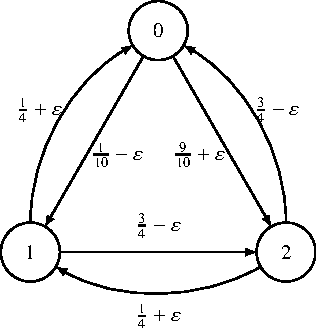
\includegraphics{chapters/80-wahrscheinlichkeit/images/spielBtilde.pdf}
\caption{Zustandsdiagramm für das modifizerte Spiel $\tilde{B}$,
Zustände sind die Dreierreste des Kapitals.
Gegenüber dem Spiel $B$
(Abbildung~\ref{buch:wahrscheinlichkeit:fig:spielB})
sind die Wahrscheinlichkeiten für Verlust 
um $\varepsilon$ vergrössert und die Wahrscheinlichkeiten für Gewinn um
$\varepsilon$ verkleinert worden.
\label{buch:wahrscheinlichkeit:fig:spielBtile}}
\end{figure}
%
Wir modifizieren jetzt das Spiel $B$ derart, dass die Wahrscheinlichkeiten
für Gewinn um $\varepsilon$ verringert werden und die Wahrscheinlichkeiten
für Verlust um $\varepsilon$ vergrössert werden.
Die Übergangsmatrix des modifzierten Spiels $\tilde{B}$ ist
\[
\tilde{B}
=
\begin{pmatrix}
 0                       & \frac{1}{4}+\varepsilon & \frac{3}{4}-\varepsilon \\
\frac{1}{10}-\varepsilon & 0                       & \frac{1}{4}+\varepsilon \\
\frac{9}{10}+\varepsilon & \frac{3}{4}-\varepsilon & 0
\end{pmatrix}
=
B
+
\varepsilon
\underbrace{
\begin{pmatrix}
 0& 1&-1\\
-1& 0& 1\\
 1&-1& 0
\end{pmatrix}
}_{\displaystyle F}
\]
Wir wissen bereits, dass der Vektor $p$
von \eqref{buch:wahrscheinlichkeit:spielBP}
als stationäre Verteilung
Eigenvektor zum Eigenwert
$B$ ist, wir versuchen jetzt in erster Näherung die modifizierte
stationäre Verteilung $p_{\varepsilon}=p+\varepsilon p_1$ des modifizierten
Spiels zu bestimmen.

\subsubsection{Gewinnerwartung im modifizierten Einzelspiel}
Die Gewinnerwartung aus den verschiedenen Ausgangszuständen kann mit Hilfe
des Hadamard-Produktes berechnet werden.
Wir berechnen dazu zunächst
\[
G\odot \tilde{B}
=
G\odot (B+\varepsilon F)
=
G\odot B + \varepsilon G\odot F
\quad\text{mit}\quad
G\odot F = \begin{pmatrix}
0&1&1\\
1&0&1\\
1&1&0
\end{pmatrix}.
\]
Nach der früher dafür gefundenen Formel ist
\begin{align*}
\begin{pmatrix}
E(Y|K\equiv 0)&
E(Y|K\equiv 1)&
E(Y|K\equiv 2)
\end{pmatrix}
&=
U^t (G\odot \tilde{B})
\\
&=
U^t (G\odot B)
+
\varepsilon
U^t (G\odot F)
\\
&=
\begin{pmatrix} -\frac{8}{10}&\frac12&\frac12 \end{pmatrix}
+
2\varepsilon U^t
\\
&=
\begin{pmatrix} -\frac{8}{10}+2\varepsilon&\frac12+2\varepsilon&\frac12+2\varepsilon \end{pmatrix}.
\end{align*}
Unter der Annahme gleicher Wahrscheinlichkeiten für die Ausgangszustände,
erhält man die Gewinnerwartung
\begin{align*}
E(Y)
&=
U^t(G\odot \tilde{B})
\begin{pmatrix}
\frac13\\
\frac13\\
\frac13
\end{pmatrix}
\\
&=
U^t
(G\odot B)
\frac13 U
+
\varepsilon
U^t
(G\odot F)
\frac13 U
\\
&=
\frac1{15}
+
2\varepsilon
\end{align*}
unter Verwendung der in
\eqref{buch:wahrscheinlichkeit:eqn:BodotEinzelerwartung}
berechneten Gewinnerwartung für das Spiel $B$.

\subsubsection{Iteration des modifizierten Spiels}
Der Gaussalgorithmus liefert nach einiger Rechnung, die man am besten
mit einem Computeralgebrasystem durchführt,
\[
\begin{tabular}{|>{$}c<{$}>{$}c<{$}>{$}c<{$}|}
\hline
-1                       & \frac{1}{4}+\varepsilon & \frac{3}{4}-\varepsilon \\
\frac{1}{10}-\varepsilon & -1                      & \frac{1}{4}+\varepsilon \\
\frac{9}{10}+\varepsilon & \frac{3}{4}-\varepsilon & -1                      \\
\hline
\end{tabular}
\rightarrow
%                [           2                   ]
%                [ 80 epsilon  + 12 epsilon + 78 ]
%(%o15)  Col 1 = [                               ]
%                [               0               ]
%                [                               ]
%                [               0               ]
%         [               0               ]
%         [                               ]
% Col 2 = [           2                   ]
%         [ 80 epsilon  + 12 epsilon + 78 ]
%         [                               ]
%         [               0               ]
%         [              2                    ]
%         [ (- 80 epsilon ) + 40 epsilon - 65 ]
%         [                                   ]
% Col 3 = [              2                    ]
%         [ (- 80 epsilon ) - 12 epsilon - 26 ]
%         [                                   ]
%         [                 0                 ]
\begin{tabular}{|>{$}c<{$}>{$}c<{$}>{$}c<{$}|}
\hline
1&0&-\frac{65-40\varepsilon+80\varepsilon^2}{78+12\varepsilon+80\varepsilon^2}\\
0&0&-\frac{26+12\varepsilon+80\varepsilon^2}{78+12\varepsilon+80\varepsilon^2}\\
0&0&0\\
\hline
\end{tabular},
\]
woraus man die Lösung
\[
p
=
\begin{pmatrix}
65-40\varepsilon+80\varepsilon^2\\
26+12\varepsilon+80\varepsilon^2\\
78+12\varepsilon+80\varepsilon^2\\
\end{pmatrix}
\]
ablesen kann.
Allerdings ist dies keine Wahrscheinlichkeitsverteilung,
wir müssen dazu wieder normieren.
Die Summe der Komponenten ist
\[
\|p\|_1
=
169 - 16 \varepsilon + 240 \varepsilon^2.
\]
Damit bekommen wir für die Lösung bis zur ersten Ordnung
\[
p_\varepsilon
=
\frac{1}{ 169 - 16 \varepsilon + 240 \varepsilon^2}
\begin{pmatrix}
65-40\varepsilon+80\varepsilon^2\\
26+12\varepsilon+80\varepsilon^2\\
78+12\varepsilon+80\varepsilon^2\\
\end{pmatrix}
=
%          [                                 2                   3         ]
%          [ 5    440 epsilon   34080 epsilon    17301120 epsilon          ]
%          [ -- - ----------- - -------------- + ----------------- + . . . ]
%          [ 13      2197           371293           62748517              ]
%          [                                                               ]
%          [                                 2                  3          ]
%(%o19)/T/ [ 2    188 epsilon   97648 epsilon    6062912 epsilon           ]
%          [ -- + ----------- + -------------- - ---------------- + . . .  ]
%          [ 13      2197           371293           62748517              ]
%          [                                                               ]
%          [                                 2                   3         ]
%          [ 6    252 epsilon   63568 epsilon    11238208 epsilon          ]
%          [ -- + ----------- - -------------- - ----------------- + . . . ]
%          [ 13      2197           371293           62748517              ]
\frac{1}{13}
\begin{pmatrix} 5\\2\\6 \end{pmatrix}
+
\frac{\varepsilon}{2197}
\begin{pmatrix}
-440\\188\\252
\end{pmatrix}
+
O(\varepsilon^2).
\]
Man beachte, dass der konstante Vektor der ursprüngliche Vektor $p$
für das Spiel $B$ ist.
Der lineare Term ist ein Vektor, dessen Komponenten sich zu $1$ summieren,
in erster Ordnung ist also die $l^1$-Norm des Vektors wieder 
$\|p_\varepsilon\|_1=0+O(\varepsilon^2)$.

Mit den bekannten Wahrscheinlichkeiten kann man jetzt die
Gewinnerwartung in einem einzeln Spiel ausgehend von der Verteilung
$p_{\varepsilon}$ berechnen.
Dazu braucht man das Hadamard-Produkt
\[
G\odot \tilde{B}
=
G=\begin{pmatrix}
 0&-1& 1\\
 1& 0&-1\\
-1& 1& 0
\end{pmatrix}
\odot
\begin{pmatrix}
0                        &\frac14+\varepsilon & \frac34-\varepsilon \\
\frac{1}{10}-\varepsilon & 0                  & \frac14+\varepsilon \\
\frac{9}{10}+\varepsilon &\frac34-\varepsilon & 0
\end{pmatrix}
=
\begin{pmatrix}
 0                        &-\frac14-\varepsilon & \frac34-\varepsilon \\
 \frac{1}{10}-\varepsilon & 0                   &-\frac14-\varepsilon \\
-\frac{9}{10}-\varepsilon & \frac34-\varepsilon & 0
\end{pmatrix}
\]
Wie früher ist der erwartete Gewinn
\begin{align*}
E(Y)
&=
U^t (G\odot \tilde{B}) p_{\varepsilon}
\\
&=
\begin{pmatrix}
-\frac{3}{10}-2\varepsilon & \frac12-2\varepsilon & \frac12-2\varepsilon
\end{pmatrix}
p_{\varepsilon}
\\
%                               3             2
%                    480 epsilon  - 48 epsilon  + 294 epsilon
%(%o50)            - ----------------------------------------
%                                   2
%                        240 epsilon  - 16 epsilon + 169
&=
-
\varepsilon\cdot
\frac{
294-48\varepsilon+480\varepsilon^2
}{
169-16\varepsilon+240\varepsilon^2
}
=
-\frac{294}{169}\varepsilon + O(\varepsilon^2).
\end{align*}
Insbesondere ist also die Gewinnerwartung negativ für nicht zu grosse 
$\varepsilon>0$.
Das Spiel ist also ein Verlustspiel.

%
% Die Kombination
%
\subsection{Kombination der Spiele
\label{buch:subsection:kombination}}
Jetzt werden die beiden Spiele $A$ und $B$ zu einem neuen
Spiel kombiniert.
Für das Spiel $A$ haben wir bis jetzt keine Übergansmatrix aufgestellt,
da das Kapital darin keine Rolle spielt.
Um die beiden Spiele kombinieren zu können brauchen wir aber die Übergansmatrix
für die drei Zustände $K\equiv 0,1,2$.
Sie ist
\[
A=\begin{pmatrix}
0&\frac12&\frac12\\
\frac12&0&\frac12\\
\frac12&\frac12&0
\end{pmatrix}.
\]

\subsubsection{Das Spiel $C$}
In jeder Durchführung des Spiels wird mit einem Münzwurf entschieden,
ob Spiel $A$ oder Spiel $B$ gespielt werden soll.
Mit je Wahrscheinlichkeit $\frac12$ werden also die Übergansmatrizen
$A$ oder $B$ verwendet:
\[
P(K\equiv i|K\equiv j)
=
A\cdot P(\text{Münzwurf Kopf})
+
B\cdot P(\text{Münzwurf Kopf})
=
\frac12(A+B)
=
\begin{pmatrix}
0            & \frac{3}{8} & \frac{5}{8} \\
\frac{3}{10} & 0           & \frac{3}{8} \\
\frac{7}{10} & \frac{5}{8} & 0
\end{pmatrix}
\]
Die Gewinnerwartung in einem Einzelspiel ist
\begin{align*}
E(Y)
&=
U^t
(G\odot C)
\frac13U
\\
&=
U^t
\begin{pmatrix}
 0            &-\frac{3}{8} & \frac{5}{8} \\
 \frac{3}{10} & 0           &-\frac{3}{8} \\
-\frac{7}{10} & \frac{5}{8} & 0
\end{pmatrix}
\frac13U
\\
&=
\begin{pmatrix}
-\frac{2}{5} & \frac{1}{4} & \frac{1}{4}
\end{pmatrix}
\frac13U
=
\frac13\biggl(-\frac{2}{5}+\frac{1}{4}+\frac{1}{4}\biggr)
=
-\frac{1}{30}
\end{align*}
Das Einzelspiel ist also ein Verlustspiel.

\subsubsection{Das iterierte Spiel $C$}
Für das iterierte Spiel muss man wieder den Eigenvektor von $C$ zum
Eigenwert $1$ finden, die Rechnung mit dem Gauss-Algorithmus liefert
\[
p=
\frac{1}{709}
\begin{pmatrix}
245\\180\\284
\end{pmatrix}.
\]
Damit kann man jetzt die Gewinnwahrscheinlichkeit im iterierten Spiel
berechnen, es ist
\begin{align*}
E(Y)
&=
U^t
(G\odot C) p
\\
&=
\begin{pmatrix}
-\frac{2}{5} & \frac{1}{4} & \frac{1}{4}
\end{pmatrix}
\frac{1}{709}
\begin{pmatrix}
245\\180\\84
\end{pmatrix}
\\
&=
\frac{
-2\cdot 49 + 45 + 71
}{709}
=
\frac{18}{709},
\end{align*}
Das iteriert Spiel $B$ ist also ein Gewinnspiel!
Obwohl die Spiele $A$ und $B$ für sich alleine in der iterierten Form
keine Gewinnspiele sind, ist das kombinierte Spiel, wo man zufällig
die beiden Spiel verbindet immer ein Gewinnspiel.

Man kann statt des Spiels $B$ auch das modifizierte Spiel $\tilde{B}$ 
verwenden, welches für kleine $\varepsilon>0$ ein Verlustspiel ist.
Die Analyse lässt sich in der gleichen Weise durchführen und liefert
wieder, dass für nicht zu grosses $\varepsilon$ das kombinierte Spiel
ein Gewinnspiel ist.





